\documentclass[aspectratio=1610]{beamer}
\usepackage{makecell}
\usepackage{graphicx}
\graphicspath{{fig/}}         
\usepackage{relsize}
\usepackage{amssymb}
\usepackage{hyperref}
\usepackage{natbib}
\usepackage{grffile}
\usepackage{amsmath}  
\usepackage{subcaption}
\usepackage[font=footnotesize,labelfont=bf]{caption}
\usepackage[font=footnotesize,labelfont=bf]{subcaption}
\usepackage{color}
\usepackage[]{algorithm2e}
\usepackage[utf8]{inputenc}
\usepackage[english]{babel}
\usepackage[toc,page]{appendix}
\usepackage{tikz}
\usetikzlibrary{arrows,backgrounds,calc,trees}
\tikzset{multiline/.style={align=center,anchor=north}}
\usepackage{ifthen}
\usetikzlibrary{positioning}
\usepackage{siunitx}
\usepackage{datatool}
\usepackage{booktabs}
\usepackage{rotating}
\usepackage{bm}
\usepackage{tabularx}
\usepackage{mathtools}
\usepackage{xcolor}
\usepackage{url}
\usepackage{qrcode}
\usepackage{bm}
\usepackage{bbm}
\usepackage{amssymb}
\usepackage{ marvosym }
\usepackage{bbold}
\usepackage{wasysym}
\usepackage{svg}
\usepackage{qrcode}
\usepackage[makeroom]{cancel}
\usepackage{comment}
\usepackage{pgfplots}
\usepgfplotslibrary{fillbetween}
\pgfplotsset{compat=1.18}
\usetikzlibrary{decorations.pathreplacing}

\usepackage{amsmath}
\usepackage{pgfplots}
\pgfplotsset{compat=1.18}

\usetikzlibrary{positioning}
\tikzset{
    neuron/.style={circle, draw, minimum size=0.4cm, inner sep=0pt},
    layer/.style={draw=none, fill=none, align=center},
    arrow/.style={-latex, thick}
}

\beamertemplatenavigationsymbolsempty
\setbeamertemplate{footline}[frame number]

\newcommand{\backupbegin}{
   \newcounter{framenumberappendix}
   \setcounter{framenumberappendix}{\value{framenumber}}
}
\newcommand{\backupend}{
   \addtocounter{framenumberappendix}{-\value{framenumber}}
   \addtocounter{framenumber}{\value{framenumberappendix}} 
}


\newcommand{\x}{\mathbf{x}}
\newcommand{\g}{\mathbf{g}}
\newcommand{\m}{\mathbf{m}}
\newcommand{\f}{\mathbf{f}}
\newcommand{\nn}{\mathcal{N}_{\bm{\rho}}}
\newcommand{\kb}{\mathbf{k}}
\newcommand{\dtr}{\mathcal{D}_{\text{train}}}
\newcommand{\birth}{\text{birth}}
\newcommand{\lr}{\alpha_{\text{learn}}}
\newcommand{\bff}{\textbf{f}}
\newcommand{\eg}{\emph{e.g.}}
\newcommand{\R}{\mathbb{R}}
\newcommand{\E}[1]{{\text{E}\left[ #1 \right]}}
\newcommand{\Eind}[2]{{\text{E}_{#1}\left[ #2 \right]}}
\newcommand{\Eaggt}[1]{\text{E}^{\text{agg}}_t\left[#1 \right]}
\newcommand{\biground}[1]{{\left( #1 \right)}}
\newcommand{\ct}{\tilde{c}}

\newcommand{\phif}[1]{\phi \left(#1 \right)}
\newcommand{\phiprf}[1]{\phi'\left(#1 \right)}
\newcommand{\sagg}{s^{\text{agg}}}
\newcommand{\snagg}{\tilde{s}^{\text{agg}}}
\newcommand{\Vf}{V^{\text{firm}}}
\newcommand{\bigrext}[1]{\left[#1\right]}

\definecolor{uzhblue}{RGB}{0,40,165}
\definecolor{uzhbluedark}{RGB}{0,32,132}

\definecolor{uzhgreydark}{RGB}{81.5,86.5,94}
\definecolor{uzhgrey}{RGB}{163,173,186}
%\definecolor{uzhgreylight}{RGB}{209,214,220.5}
%\definecolor{uzhgreylight}{RGB}{227.4,230.4,234.3}
\definecolor{uzhgreylight}{RGB}{236.6,238.6,241.2}

\definecolor{uzhorange}{RGB}{220,96,39}
\def\checkmark{\tikz\fill[scale=0.4](0,.35) -- (.25,0) -- (1,.7) -- (.25,.15) -- cycle;} 



\usepackage{appendixnumberbeamer}




\usecolortheme{dove}
\setbeamerfont{frametitle}{size=\huge}





\DeclareMathOperator*{\argmax}{arg\,max}
\DeclareMathOperator*{\argmin}{arg\,min}



\definecolor{myred}{rgb}{200, 0.0, 0.25}
\definecolor{uzhblue}{rgb}{0, 0, 0.5}

\definecolor{upennblue}{RGB}{1,31,91}
\definecolor{harvardcrimson}{RGB}{153,0,0}

\newcommand{\emphc}[1]{\textcolor{harvardcrimson}{#1}}



\hypersetup{colorlinks,linkcolor={harvardcrimson},citecolor={uzhgreydark},urlcolor={harvardcrimson}} 

\setbeamercolor{frametitle}{bg=uzhgreylight, fg = uzhblue}

\newcommand{\blup}[1]{\textcolor{uzhgreydark}{#1}} 

\makeatletter
\let\@citexOld\@citex
\def\@citex[#1]#2{\blup{\@citexOld[#1]{#2}}}
\makeatother

\let\citeOld\cite % renew cite
\renewcommand{\cite}[1]{{\blup{\citeOld{#1}}}}
\let\citetOld\citet % renew cite
\renewcommand{\citet}[1]{{\blup{\citetOld{#1}}}}

\def\layersep{2.5cm}


\pgfdeclarelayer{background}
\pgfsetlayers{background,main}



%*-*-*-*-*-*-*-*-*-*-*-*-*-*-*-*-*-*-*-*-*-*


\setbeamercolor*{title}{fg=uzhblue}   

%%%%%%%%%%%%%%%%%%%%%%%%%%%%%%%%%%%%%%%%%%%%%%%%%%%%%



\title[Deep Learning for Dynamic Economic Models]{Deep Learning for Economics and Finance}
\subtitle{Stochastic IAMs with DEQNs, GP surrogates, Sobol sensitivity indices, constrained Pareto-improving carbon-tax design}
\author{Simon Scheidegger}
\institute[HEC Lausanne]{HEC, University of Lausanne}
\date{}



%%%%%%%%%%%%%%%%%%%%%%%%%%%%%%%%%%%%%%%%%%%%%%%%%%%%%

\begin{document}

%%%%%%%%%%%%%%%%%%%%%%%%%%%%%%%%%%%%%%%%%%%%%%%%%%%%%
{\setbeamercolor{background canvas}{bg=uzhgreylight}
\begin{frame}
\titlepage
\vspace{-0.4cm}
\begin{center}
{\footnotesize Based on: K\"ubler, Scheidegger \& Surbek (2026, forthcoming, \textit{JPE: Macroeconomics}; arXiv:2507.01704)}\\[2pt]
{\footnotesize Companion code: \url{https://github.com/sischei/JPE_Macro_Using_ML_to_compute_constrained_optimal_carbon_tax_rules}}\\[4pt]
{\footnotesize Materials: \url{https://github.com/sischei/Deep_Learning_for_Solving_And_Estimating_Dynamic_Economic_Models}}
\end{center}
\end{frame}
}
%%%%%%%%%%%%%%%%%%%%%%%%%%%%%%%%%%%%%%%%%%%%%%%%%%%%%

    \begin{comment}
\begin{frame}{Outline of the Talk}

% FK:  Would delete this for 20 min talk

    \setbeamertemplate{section in toc}[sections numbered]
  \tableofcontents%[hideallsubsections]  

\end{frame}
\end{comment}



%%%%%%%%%%%%%%%%%%%%%%%%%%%%%%%%%%%%%%%%%%%%%%%%%%%%%
%%%%%%%%%%%%%%%%%%%%%%%%%%%%%%%%%%%%%%%%%%%%%%%%%%%%%
%\section[Introduction]{Introduction}

%%%%%%%%%%%%%%%%%%%%%%%%%%%%%%%%%%%%%%%%%%%%%%%%%%%%%
%%%%%%%%%%%%%%%%%%%%%%%%%%%%%%%%%%%%%%%%%%%%%%%%%%%%%

%%%%%%%%%%%%%%%%%%%%%%%%%%%%%%%%%%%%%%%%%%%%%%%%%%%%%%%%%%%%%%


\begin{frame}{The Challenge: Climate Risk \& Heterogeneity}

    \begin{columns}[c] % Vertically centered columns
    
        % --- Left Column: Visuals ---
        \begin{column}{0.45\textwidth}
            \centering
            % Image 1: Temperature Anomaly
            \includegraphics[width=0.95\linewidth]{temperature-anomaly.png}
            
            \vspace{0.5em} % Spacing between images
            
            % Image 2: Global Warming (Disasters)
            \includegraphics[width=0.95\linewidth]{global-warming.png}
        \end{column}

        % --- Right Column: Key Points ---
        \begin{column}{0.55\textwidth}
            \small % Slightly smaller font to fit comfortably
            \begin{itemize}
                \setlength\itemsep{1em} % Good spacing between bullets
                
                \item \textbf{Systemic Risk:} Climate change poses a fundamental threat to global economic stability and human welfare.
                
                \item \textbf{Non-Linear Dynamics:} Tipping points introduce the risk of irreversible, catastrophic environmental shifts.
                
                \item \textbf{Distributional Impact:} Effects will be highly heterogeneous, creating profound equity challenges across regions and generations.
                
                \item \textbf{Literature Context:} These macro-financial linkages are detailed in the recent review Fernandez-Villaverde, Gillingham, and Scheidegger (2025).
            \end{itemize}
        \end{column}
        
    \end{columns}

\end{frame}

\begin{comment}
    
\begin{frame}[fragile]{Climate Change}

\begin{figure*}
 \centering
  \includegraphics[width=0.39\textwidth]{temperature-anomaly.png}
 \includegraphics[width=0.6\textwidth]{global-warming.png}  
  \label{global-problem}
    \end{figure*} 

\begin{itemize}
   % \item Climate Change: One of the Planet’s worst externality.
    %\item Likely to reduce future global GDP by one third.
    \item Global warming is a growing threat (to economic well being,...).
    \item Portends massive human suffering.
    \item Tipping points place us in catastrophic danger.
     \item It will impact current and future generations in different regions in very different ways.
     \item A recent review by Fernandez-Villaverde, Gillingham, and Scheidegger (2025).
\end{itemize}

  \end{frame}
\end{comment}


%%%%%%%%%%%%%%%%%%%%%%%%%%%%%%%%%%%%%%%%%%%%%%%%%%%%%
\begin{frame}{Motivation: Designing Optimal Policy}

    \begin{itemize}
        \setlength\itemsep{1.5em}
        
        \item \textbf{The Consensus:} Carbon pricing is widely regarded as the most efficient tool to mitigate emissions.
        
        \item \textbf{The Difficulty:} In a world with heterogeneous agents (e.g., OLG), simple taxes create winners and losers, threatening political feasibility.
        
        \item \textbf{The Objective:} We need a systematic way to compute \textcolor{blue}{constrained optimal taxes} that:
        \begin{itemize}
            \item Account for stochastic risks (tipping points).
            \item Respect political constraints (Pareto improvements).
        \end{itemize}
    \end{itemize}

\end{frame}

\begin{comment}
    
\begin{frame}{Motivation}

\begin{itemize}
    \item Can economic policy mitigate climate change?
    \vspace{0.5cm}
    \begin{itemize}
    \item Regulation
    \item R \& D subsidies
    \item Carbon taxes
    \item Other subsidies
    \end{itemize}
    \vspace{0.5cm}
    \item \textcolor{blue}{Need a systematic way to compute (constrained) optimal taxes in stochastic environments with heterogeneous agents.}
\end{itemize}         
        
\end{frame}
\end{comment}

  
%%%%%%%%%%%%%%%%%%%%%%%%%%%%%%%%%%%%%%%%%%%%%%%%%%%%%

\begin{comment}
    
\begin{frame}[fragile]{Welfare Analysis - Heterogeneous Agents}

\begin{figure}
    \centering
    \includegraphics[width=0.49\linewidth]{olg_agents.jpg}
    \includegraphics[width=0.49\linewidth]{quote.png}
    \caption{Overlapping Generations.}
    \label{fig:enter-label}
\end{figure}

%\begin{footnotesize}
\begin{itemize}
    \item Current research in climate change macro often resorts to \textcolor{blue}{simplifying assumptions} (e.g., representative agent) or searches for Pareto improvements by \textcolor{blue}{guessing}.

    \item Want to develop systematic tools for optimal policy within \textcolor{blue}{globally solved} models that take into account \textcolor{blue}{heterogeneity and stochasticity}. 

\end{itemize}
%\end{footnotesize}
\end{frame}
\end{comment}
\begin{frame}[fragile]{The Gap: Welfare Analysis in Stochastic OLG IAMs}

    % Figure placement preserved exactly as requested
    \begin{figure}
        \centering
        \includegraphics[width=0.49\linewidth]{olg_agents.jpg}
        \includegraphics[width=0.49\linewidth]{quote.png}
        \caption{Overlapping Generations.}
        \label{fig:enter-label}
    \end{figure}

    \vspace{-0.2cm}

    \begin{itemize}
        \setlength\itemsep{1em}
        
        \item \textbf{Current Limitations:} Most climate-macro research relies on \textcolor{blue}{simplifying assumptions} (e.g., representative agents) or heuristic "guessing" to find Pareto improvements.

        \item \textbf{The Missing Tool:} A framework for \textcolor{blue}{global solutions} in high-dimensional, stochastic environments that explicitly handles:
        \begin{itemize}
            \item \textbf{Heterogeneity:} Winners vs. Losers.
            \item \textbf{Uncertainty:} Tipping points and damage shocks.
        \end{itemize}

    \end{itemize}
\end{frame}

%%%%%%%%%%%%%%%%%%%%%%%%%%%%%%%%%%%%%%%%%%%%%%%%%%%%
\begin{frame}[fragile]{Our Contribution: A Scalable Policy Framework}

    \begin{columns}[t]
    
        % Left Column
        \begin{column}{0.5\textwidth}
            \textbf{1. The Method} 
            
            \vspace{0.5em}
            \centering
            \includegraphics[width=0.95\linewidth]{flow_chart_2.png}
            
            \vspace{0.5em}
            \raggedright
            \small{A 3-step ML pipeline to alleviate the \textcolor{blue}{curse of dimensionality}.}
        \end{column}

        % Right Column
        \begin{column}{0.5\textwidth}
            \textbf{2. The Application}
            
            \vspace{0.2em}
            \small
            We compute the first \textcolor{blue}{globally optimal, Pareto-improving carbon tax} in a stochastic OLG model with tipping points.
            
            \vspace{1.5em}
            
            \textbf{3. A Generic Blueprint}
            
            \vspace{0.2em}
            A universal framework for \textbf{almost any} stochastic heterogeneous-agent model. It allows researchers to both \textcolor{blue}{solve global equilibria} and derive \textcolor{blue}{constrained-optimal policies} in settings previously deemed intractable.
        \end{column}
        
    \end{columns}

\end{frame}
%%%%%%%%%%%%%%%%%%%%%%%%%%%%%%%%%%%%%%%%%%%%%%%%%%%%%

\begin{comment}
    
\begin{frame}[fragile]{An Incomplete List of Related Literature}

% FK:  Would delete this for 20 min talk

\begin{small}
\begin{itemize}
   % \item {\bf{Literature on climate change and integrated assessment models}} (see, e.g,~\cite{Nordhaus_1979, Nordhaus2017}).
    \item {\bf{Literature on (stochastic) OLG models with global warming}:} e.g.,~\cite{kotlikoff2021making}, \cite{kotlikoffParetoimprovingCarbonriskTaxation2021a}, and~\cite{Karp2024}.
            \vspace{0.5cm}
    % \item {\bf{Literature on calculating Pareto frontier}:}  e.g.,~\cite{bakerBigDataApproach2014}.
            % \vspace{0.5cm}
    \item {\bf Optimal Ramsey taxation with heterogenous agents:} e.g.,~\cite{dyrda2023optimal}, \cite{bhandari2013taxes}, \cite{feng2024optimal}.
\end{itemize}
\end{small}

\end{frame}
\end{comment}
\begin{frame}{An Incomplete List of Related Literature}
    \small
    
    % Block 1: The Economic Challenge
    \begin{block}{Climate Risk in OLG Models}
        Existing work studies intergenerational conflict and climate damages \citep{kotlikoff2021making, weitzman2012ghg, Karp2014}.
        \begin{itemize}
            \item[\textcolor{blue}{\textbf{+}}] \textbf{Our Gap:} Most rely on linearization or ignore the \textit{political constraint} of Pareto improvements under uncertainty (e.g., tipping points).
        \end{itemize}
    \end{block}

    % Block 2: The Policy Framework
    \begin{block}{Optimal Ramsey Policy with Heterogeneity}
        Established frameworks for fiscal/monetary policy in HA models \citep{bhandari2013taxes, nuno2020Optimal, douenne_hummel_pedroni_2024}.
        \begin{itemize}
             \item[\textcolor{blue}{\textbf{+}}] \textbf{Our Gap:} We enforce \textit{simple rules} (linear taxes) to make the policy implementable and interpretable.
        \end{itemize}
    \end{block}

    % Block 3: The Computational Solution
    \begin{block}{Deep Learning for High-Dimensional Dynamic Stochastic Models}
        Using Neural Networks (DEQN) and Surrogates to beat the curse of dimensionality \citep{azinovic_et_al_2019, friedlDeep2023}.
        \begin{itemize}
             \item[\textcolor{blue}{\textbf{+}}] \textbf{Our Innovation:} A 3-step framework: DEQN (Global Solution) $\to$ GP Surrogate $\to$ Constrained Optimization.
        \end{itemize}
    \end{block}
\end{frame}
%%%%%%%%%%%%%%%%%%%%%%%%%%%%%%%%%%%%%%%%%%%%%%%%%%%%%

%%%%%%%%%%%%%%%%%%%%%%%%%%%%%%%%%%%%%%%%%%%%%%%%%%%%%%%%%%%%%%%
\begin{frame}{Outline of this talk}
  \setbeamertemplate{section in toc}[sections numbered]
  \tableofcontents%[hideallsubsections]
\end{frame}


\section[Model]{Model}
%%%%%%%%%%%%%%%%%%%%%%%%%%%%%%%%%%%%%%%%%%%%%%%%%%%%%

%%%%%%%%%%%%%%%%%%%%%%%%%%%%%%%%%%%%%%%%%%%%%%%%%%%%%


    {\setbeamercolor{background canvas}{bg=uzhgreylight}
\begin{frame}
\Huge \textcolor{uzhblue}{Our Model}
%\begin{figure}
%    \centering
%    \includegraphics[width=0.5\textwidth]{IAM.png}
%    \caption{Caption}
%    \label{fig:enter-label}
%\end{figure}
\end{frame}}

%%%%%%%%%%%%%%%%%%%%%%%%%%%%%%%%%%%%%%%%%%%%%%%%%%%%%

\begin{frame}
\frametitle{Integrated Assessment Models (IAMs)}

\begin{itemize}
\item Pioneered by Nordhaus (DICE, RICE): Quantitative, often numerical.
\item Key components:
\begin{itemize}
    \item (Simplified) climate system.
    %\item (Stylized) carbon cycle.
    \item (Stylized) economic model of emissions AND damages.
\end{itemize}

\item Economic model: needs to be dynamic, forward-looking, possibly allowing stochasticity (temperature variations, disasters, TFP), and potentially heterogeneous agents (``who is how impacted?'').
\end{itemize}
\vfill
%%%%%%%%%%%%%%%%%%%%%%%%%%%%%%%%%%%%%%%%%%%%%%%%%%%%%%%%%%%%%%%
%
\begin{figure}[h]
\centering
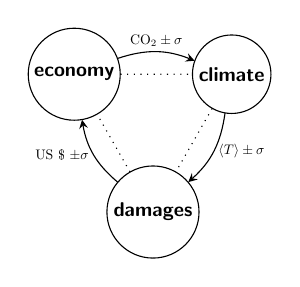
\begin{tikzpicture}[>=stealth, node distance=2cm, scale=0.5, transform shape]
    % Define style for the nodes
    \tikzstyle{main node} = [circle, draw, minimum size=1cm, font=\sffamily\Large\bfseries]
    
    % Nodes
    \node[main node] (economy) at (0,0) {economy};
    \node[main node] (climate) at (4,0) {climate};
    \node[main node] (damages) at (2,-3.5) {damages};
    
    % Arrows with labels
    \draw[->] (economy) to[bend left=20] node[above] {CO$_2 \pm \sigma$} (climate);
    \draw[->] (climate) to[bend left=20] node[right] {$\langle T \rangle \pm \sigma$} (damages);
    \draw[->] (damages) to[bend left=20] node[left] {US \$ $\pm \sigma$} (economy);
    
    % Triangle
    \draw[dotted] (economy) -- (climate) -- (damages) -- (economy);

\end{tikzpicture}
\caption{Stylized representation of an IAM.}
\label{fig:IAM_stylized}
\end{figure}

%%%%%%%%%%%%%%%%%%%%%%%%%%%%%%%%%%%%%%%%%%%%%%%%%%%%%%%%%%%%%%%
\end{frame}

%HERERERERE

\begin{frame}[fragile]{Overview of our Stochastic IAM}

\begin{itemize}
    \item 12 Overlapping generations of selfish agents.
            \vspace{0.5cm}
    \item 5-yearly-calibrated model: agents live from age 20 to age 80.
            \vspace{0.5cm}
    \item Use a simple climate module~\citep{Dietz2020}.
            \vspace{0.5cm}
    \item Use a damage function with stochastic tipping~\citep{kotlikoffParetoimprovingCarbonriskTaxation2021a}.
            \vspace{0.5cm}
    \item Exogenously declining carbon intensity as in DICE-2016~\citep{nordhaus2017revisiting}.
\end{itemize}

\end{frame}

%%%%%%%%%%%%%%%%%%%%%%%%%%%%%%%%%%%%%%%%%%%%%%%%%%%%%

%%%%%%%%%%%%%%%%%%%%%%%%%%%%%%%%%%%%%%%%%%%%%%%%%%%%%%%%%%%%%%%%%%%%%
\subsection*{Technology}
\label{sec:firms}
%%%%%%%%%%%%%%%%%%%%%%%%%%%%%%%%%%%%%%%%%%%%%%%%%%%%%%%%%%%%%%%%%%%%%

\begin{frame}[fragile]{Technology}
\begin{footnotesize}

\textcolor{blue}{Firms}, in each period, $t$, produce \textcolor{blue}{final output, $Y_{t}$, and emissions $e_t$ with capital, $K_{t}$ and labor, $L_{t}$}, and choose how much of its emissions to \textcolor{blue}{mitigate $\mu_t$} according to 
%
\begin{equation} \label{eqFinalOutput} 
(Y_t, e_t) = (\Omega_t(T_{t}) \Phi(\mu_t)
 K_t^{\alpha} L_t^{1-\alpha} + (1- \delta) K_t, \; \kappa_t (1-\mu_t)
 K_t^{\alpha} L_t^{1-\alpha})
\end{equation}
%
\begin{footnotesize}
    \begin{itemize}
\item $\Omega_t(T_{t})$: climate damages that reduce output.
\item $\Phi(\mu_t)$ is a mitigation cost function.
\item $\alpha$ is the capital share.
\item $\kappa_t$ is carbon intensity. We assume that $\kappa_t$ decreases stochastically over time as in \cite{kotlikoffParetoimprovingCarbonriskTaxation2021a}.
\item The abatement technology~\citep[{adapted from}][]{Nordhaus2017}: $\Phi(\mu_t) = (1-\theta_{1}\mu_t^{\theta_2})$.
\item $\theta_{1}$ and $\theta_2$ are parameters and $\mu_t \in [0, 1]$.
\end{itemize}
\end{footnotesize}
%$\Omega_t(T_{t})$: climate damages that reduce output, $\Phi(\mu_t)$ is a mitigation cost function, which jointly reduces emissions and output. $\alpha$ is the capital share and $\kappa_t$ is carbon intensity.

%The abatement technology, as in \cite{Nordhaus2017} takes the form: 
%\begin{equation}
%    \Phi(\mu_t) = (1-\theta_{1,t}\mu_t^{\theta_2})
%\end{equation}
%where $\theta_{1,t}$ and $\theta_2$ are parameters and $\mu_t \in [0, 1]$. The firm has to pay a tax $\tau_t$ on emissions. 
\vspace{0.5cm}
\textcolor{blue}{Profit maximization} is given by:
%\begin{equation}
%    \max_{\mu_t,K_t,L_t} \Omega_t(T_{t}) (1-\theta_1\mu_t^{\theta_2}) K_t^{\alpha} L_t^{1-\alpha} + (1- \delta) K_t -w_tL_t-(1+r_t)K_t - \tau_t (1-\mu_t) \kappa_t K_t^{\alpha} L_t^{1-\alpha}
%\end{equation}
%s.t. $0 \leq \mu_t \leq1$.

\begin{equation}
    \begin{aligned}
        \max_{\mu_t, K_t, L_t} & \quad \Omega_t(T_{t}) (1-\theta_1\mu_t^{\theta_2}) K_t^{\alpha} L_t^{1-\alpha} + (1- \delta) K_t -w_tL_t-(1+r_t)K_t - \tau_t (1-\mu_t) \kappa_t K_t^{\alpha} L_t^{1-\alpha} \\
        \text{s.t.} & \quad 0 \leq \mu_t \leq 1.
    \end{aligned}
\end{equation}


\end{footnotesize}

\end{frame}

%%%%%%%%%%%%%%%%%%%%%%%%%%%%%%%%%%%%%%%%%%%%%%%%%%%%%%%%%%%%%%%%%%%%%
\subsection*{Households}
\label{sec:households}
%%%%%%%%%%%%%%%%%%%%%%%%%%%%%%%%%%%%%%%%%%%%%%%%%%%%%%%%%%%%%%%%%%%%%

\begin{frame}[fragile]{Households}

\begin{footnotesize}

\begin{itemize}
    \item Agents enter the labor force at age 20 with 0 assets and die at age 80, after 12 periods. 
   % \item Mortality risk, which we take to be region- and year-specific, is assumed to be fully hedged via an actuarially fair annuities market.
    \item Agents born in period $t$ maximize lifetime utility:
    \begin{equation}
 {\mathbb E}_t \sum\limits_{j = 1}^{12} \beta^j \frac{C_{t+j-1, j}^{1-\sigma}}{1-\sigma} ,
\end{equation} 
\begin{equation}
\text{subject to } C_{t,j}+a_{t+1, j+1}=(1+r_t)a_{t,j} +w_{t} l_{j} + \mathbb{T}_{t,j},
\end{equation} 
where $C_{t,j}$, $a_{t,j}$, $l_{j}$ and $\mathbb{T}_{t,j}$ reference, respectively, \textcolor{blue}{consumption, asset level, labor endowment, and transfer} of those born at time $t$ who are currently age $j$.

\item $l_{j}$ is similarly calibrated as in \cite{kotlikoff2021making}. \item Agents work for 8 periods, earning labor income, and then retire. Agents aged 9 to 12 work on a 40\% basis as a proxy for a state pension system.
\item $\beta$ is the discount factor and $\sigma$ is the coefficient of relative risk aversion.
\item Welfare criterion is 
$$ U_t= {\mathbb E}_0  \sum\limits_{j = 1}^{12} \beta^j \frac{C_{t+j-1, j}^{1-\sigma}}{1-\sigma} $$
Use $ \tilde U_t $ for welfare under taxation.
\end{itemize}

\end{footnotesize}

\end{frame}

 %%%%%%%%%%%%%%%%%%%%%%%%%%%%%%%%%%%%%%%%%%%%%%%%%%%%%%%%%%%%%%%%%%%%%

\begin{frame}[fragile]{Market Clearing}
% Delete this slide, too detailed


\begin{itemize}
\item Total household assets comprise physical capital:
     \begin{equation}
    \sum_{j = 1}^{A} a_{t,j} = K_t \quad \forall t.
\end{equation}
\item Aggregate labor endowment is the sum of individual endowments:
\begin{equation}
    \sum_{j = 1}^{A} l_j = L_t \quad \forall t.
\end{equation}
\item Tax income is redistributed to households each period:
\begin{equation}
    \sum_{j=1}^{A} \mathbb{T}_{t,j} = \tau_{t} e_t \quad  \forall t .
\end{equation}


\end{itemize}



\end{frame}

%%%%%%%%%%%%%%%%%%%%%%%%%%%%%%%%%%%%%%%%%%%%%%%%%%%%%%%%%%%%%%%%%%%%%

\begin{frame}[fragile]{Redistribution of Tax Income}
    \begin{itemize}
        \item Each period's tax income is redistributed to currently alive agents.
        \item In general, \textcolor{blue}{transfer schemes may create winners and losers} \citep{kotlikoff2021making}.

        \item Today: \textcolor{blue}{2 examples of transfer policies.}
        \begin{itemize}
            \item \textcolor{blue}{``10\% scheme''}: The youngest generation receives the highest share of total tax income, with each older generation getting 10\% less than the next younger generation. Formally: $\mathbb{T}_{t,j} = 0.9^{(j-1)} \cdot 0.1394 \cdot \tau_t e_t, \quad j \in \{2,...,12 \}$.
         \vspace{0.5cm}
%             \item The alternative brute-force approach is to  search for a fixed transfer scheme for which we find a Pareto improvement ($\mathbb{T}_p$): 
    \item \textcolor{blue}{Optimal transfers}: Optimal transfer shares to each generation alive in a given period (fixed at t=0).
\end{itemize}
\end{itemize}


%     \begin{center} 
%     \footnotesize
%     \begin{tabular}{|c|c|c|c|c|c|c|c|c|c|c|c|c|}
%         \hline
%         \textbf{t1} & \textbf{t2} & \textbf{t3} & \textbf{t4} & \textbf{t5} & \textbf{t6} & \textbf{t7} & \textbf{t8} & \textbf{t9} & \textbf{t10} & \textbf{t11} & \textbf{t12} \\
%         \hline
%         0.103 & 0.093 & 0.083 & 0.083 & 0.083 & 0.093 & 0.093 & 0.093 & 0.083 & 0.083 & 0.073 & 0.033 \\
%         \hline
%     \end{tabular}
%         \end{center}

        \begin{itemize}
        \vspace{0.5cm}
        \item Normalization: Shares sum up to 1.
        % \vspace{0.5cm}
        % \item \textcolor{blue}{Preferred: find optimal transfer (but how)?}
    \end{itemize}
\end{frame}

%%%%%%%%%%%%%%%%%%%%%%%%%%%%
% OLD: 
% \begin{frame}[fragile]{Redistribution of Tax Income}
%     \begin{itemize}
%         \item Each period's tax income is redistributed to currently alive agents.
%                     \vspace{0.5cm}
%         \item In general, transfer schemes may create winners and losers \citep{kotlikoff2021making}.
%                             \vspace{0.5cm}

%         \item We aim to find Pareto improving tax/transfer schemes.
%         \vspace{0.5cm}
%         \item One current exogenous redistribution policy: The youngest generation receives the highest share of total tax income, with each older generation getting 10\% less than the next younger generation. 
%         \vspace{0.5cm}
%         \item Normalization: Shares sum to 1; that is, the youngest receives 13.94\%.
%                  \vspace{0.5cm}
%         \item formally: $\mathbb{T}_{t,j} = 0.9^{(j-1)} \cdot 0.1394 \cdot \tau_t e_t, \quad j \in \{2,...,12 \}$.
%         \item \textcolor{red}{OLI: update - add the 2 examples, T1 and T2.}
%         \vspace{0.5cm}
%         \item \textcolor{blue}{Ongoing: find optimal transfer (s.t. functional form).}
%     \end{itemize}
% \end{frame}
%%%%%%%%%%%%%%%%%%%%%%%%%%%%%%%%%%%%%%%%%%%%%%%%%%%%%%%%%%%%%%%%%%%%%
\subsection*{Modeling Climate Change's Negative Externality}
\label{sec:climate_econ}


%%%%%%%%%%%%%%%%%%%%%%%%%%%%%%%%%%%%


\begin{frame}{Cumulative Carbon Emissions and Temperature}
\scriptsize
\textbf{Overview:} Climate science shows a near-linear link between cumulative CO$_2$ emissions and global temperature rise:
\begin{itemize}
    \item Global mean temperature increase ($T^{AT}_t$) is proportional to cumulative CO$_2$ emissions ($E_s$).
    \item The proportionality constant $\sigma_{CCR}$, known as the \textcolor{blue}{Carbon-Climate Response (CCR) or TCRE}, \textcolor{blue}{ranges from 1.0 °C to 2.3 °C per 1 000 GtC (0.27 °C to 0.63 °C per 1 000 GtCO$_2$)}.
\end{itemize}

\begin{columns}[c]  % --- side-by-side layout ---------------------------------
    \column{0.4\textwidth}
        \textbf{Equation:}
        \begin{equation}
            \label{eq:agg_emission}
            T^{AT}_t \approx \sigma_{CCR} \sum_{s=0}^{t} E_s
        \end{equation}

    \column{0.52\textwidth}
        \begin{figure}
            \centering
            \includegraphics[width=0.5\linewidth]{TCRS.png}
            \caption{Figure from IPCC 6.}
            \label{fig:enter-label}
        \end{figure}
\end{columns}  % ----------------------------------------------------------------

\vspace{0.3em}
\textbf{Implications:}
\begin{itemize}
    \item Equation~\eqref{eq:agg_emission} is efficient and widely used in integrated assessment models (IAMs).
    \item It does not account for uncertainties in $\sigma_{CCR}$ nor for nonlinear effects such as potential tipping points (cf.\ Dietz and Venmans, 2019).
\end{itemize}
\end{frame}

%%%%%%%%%%%%%%%%%%%%%%%%%%%%%%%%%%%%%%%%%%%%%%%%%%%%%%%%%%%%%%%%%%%%%

\begin{frame}[fragile]{Damage Function}
\begin{small}

\begin{itemize}
    \item Damages reduce output. 
    \item We include stochastic climate tipping as in \cite{weitzman2012ghg,kotlikoffParetoimprovingCarbonriskTaxation2021a}. Climate tipping is the occurrence of climate events that lead to irreversible damage to the environment (e.g., \citealp{lenton2008tipping}).
    \item The damage function takes the following form:
    \begin{equation}
        \label{eq:damage_func_tipping}
    \Omega_t \left( T_{ t} \right) =  \frac{1}{1 + \left(\frac{1}{\psi_1} T_{ t} \right)^{2} + \left( \frac{1}{2 \cdot TP_{t}} T_{ t} \right)^{6.754}}
    \end{equation}
    %
where $\psi_1$ is a damage parameter and $TP_t$ follows a random walk which is truncated at $TP_t \in [2.5, 3.5]$. 
% where $\psi_1$ is a parameter calibrated as in \cite{Nordhaus2017} and $TP_t$ follows a random walk which is truncated at $TP_t \in [2.5, 3.5]$. 

\item Once the temperature hits a tipping point, $TP_t$ stays at the given level.

\end{itemize}



\end{small}
\end{frame}

%%%%%%%%%%%%%%%%%%%%%%%%%%%%%%%%%%%%%%%%%%%%%%%%%%%%%%%%%%%%%%%%%%%%%%%%%
\begin{frame}[fragile]{Uncertainty}
\begin{itemize}
    \item $\kappa_t$ follows an AR(1) process $\kappa_t = \rho_t \kappa_{t-1} + \epsilon_{\kappa,t}$ with $\kappa_0 = 0.3502$ and $\rho_t =  \rho_0 + (\rho_\infty - \rho_0) (1-\exp(- \delta^\rho  5t))$. 
   \item $\epsilon_{\kappa,t}$ is discretized as:  
    \begin{equation}
        \epsilon_{\kappa, t} = 
\begin{cases}
0.03 & \text{with prob } 1/3, \\
0.0 & \text{with prob } 1/3, \\
- 0.03 & \text{with prob } 1/3.
\end{cases}
    \end{equation}
    \item $TP_t$ follows a random walk $TP_t = TP_{t-1} + \epsilon_{TP,t}$ with $TP_0 = 3.0$, $\epsilon_{TP,t}$ is discretized as:
    \begin{equation}
        \epsilon_{TP, t} = 
\begin{cases}
0.1 & \text{with prob } 1/3, \\
0 & \text{with prob } 1/3, \\
- 0.1 & \text{with prob } 1/3.
\end{cases}
    \end{equation}
\end{itemize}
\end{frame}

\begin{frame}[fragile]{Equilibrium Conditions}
\begin{small}
  \begin{columns}
        % Left column
        \begin{column}{0.5\textwidth}
        \textbf{Firm:}
            \begin{align}
                0 & = \tau_t \kappa_t  - \Omega_t (T_{\mathrm{AT}, t}) \theta_1 \theta_2 \mu_t^{\theta_2 -1} \tag{$\mu_t$}\\
                %0 & = \tau_t \kappa_t - \frac{\eta_{\mu,t}}{K_t^{\alpha} L_t^{1-\alpha}} - \Omega_t (T_{\mathrm{AT}, t}) \theta_1 \theta_2 \eta_{\mu,t}^{\theta_2 -1} \tag{$\mu_t$}\\
                %0 & = \eta_{\mu,t} (1 - \mu_t) \tag{$KKT_\mu$}\\
                %0 & \leq \eta_{\mu,t} \tag{$KKT_\mu$}\\
                %0 & \leq 1 - \mu_t \tag{$KKT_\mu$}\\
                r_t & = \left( \Omega_t (T_{\mathrm{AT}, t}) (1 - \theta_1 \mu_t^{\theta_2}) \right. \notag \\
                    & \quad \left. - \tau_t \kappa_t (1 - \mu_t) \right) \alpha K_t^{\alpha - 1} L_t^{1 - \alpha} - \delta \tag{$K_t$}\\
                w_t & = \left( \Omega_t (T_{\mathrm{AT}, t}) (1 - \theta_1 \mu_t^{\theta_2}) \right. \notag\\
                    & \quad \left. - \tau_t \kappa_t (1 - \mu_t) \right) (1 - \alpha) K_t^{\alpha} L_t^{-\alpha} \tag{$L_t$}
            \end{align}
            \textbf{Households:}
            
            For all households $j \in 1,...,A-1$:
            \begin{align}
                c_t^{-\sigma}  = \beta \mathbb{E}_t \left[ (1+ r_{t+1}) c_{t+1,j+1}^{-\sigma} \right] \tag{EE} \\
                C_{t,j} + a_{t+1, j+1}  =  (1 + r_t) a_{t,j} + w_{t} l_{t,j} + \mathbb{T}_{t,j}  \tag{BC}
            \end{align}
            and initial/final conditions $a_{t,1} = 0$, $a_{t+1,A} = 0$.
        \end{column}
    
        % Right column
        \begin{column}{0.5\textwidth}
        % \textbf{Household}
        %     \begin{align}
        %         c_t^{-\sigma}  = \beta \mathbb{E}_t \left[ (1+ r_{t+1}) c_{t+1,j+1}^{-\sigma} \right] \tag{EE} \\
        %         C_{t,j} + a_{t+1, j+1}  =  (1 + r_t) a_{t,j} + w_{t} l_{t,j} + \mathbb{T}_{t,j}  \tag{BC}
        %     \end{align}
            \textbf{Market Clearing:}
            \begin{align}
                K_t & = \sum_{j = 1}^{A} a_{t,j} \tag{$K_t$}\\
            L_t & = \sum_{j = 1}^{A} l_j \tag{$L_t$} \\
            \tau_{t} e_t & = \sum_{j=1}^{A} \mathbb{T}_{t,j}  \tag{$\mathbb{T}$}
            \end{align}
        \end{column}
  \end{columns}
\end{small}
\end{frame}
%%%%%%%%%%%%%%%%%%%%%%%%%%%%%%%%%%%%%%%%%%%%%%%%%%%%%%%%%%%%%%%%%%%%%

\begin{frame}[fragile]{The Planner's Problem}

\begin{itemize}
    \setlength\itemsep{1em} 

    \item \textbf{Objective:} The planner chooses policy parameters $\vartheta$ (taxes \& transfers) to maximize the Social Welfare Function $\mathcal{W}$:
    \begin{align}
       \max_{\vartheta} \quad & \mathcal{W}(\vartheta) = \sum_{t = -10}^{30} \gamma_t \tilde{U}_t(\vartheta) \\
       \text{s.t.} \quad & \tilde{U}_t(\vartheta) \ge U_t \quad \forall t \quad \text{(if Pareto constrained)} \nonumber
    \end{align}
    \vspace{-0.5em}
    {\footnotesize \emph{(Where $\tilde{U}_t(\vartheta)$ is the ex-ante expected lifetime utility of generation $t$)}}
    
    \item \textbf{Welfare Metric:} Gains are reported as the consumption equivalence factor ($\text{CE}_t$):
    \[
       \text{CE}_t = \left(\frac{\tilde{U}_t}{U_t}\right)^{\frac{1}{1-\sigma}}-1 \quad \text{\small{(where $U_t$ is BAU utility)}}
    \]

    \item \textbf{Scope \& Challenge:} 
    \begin{itemize}
        \item Horizon: 40 generations (11 current, 29 future).
        \item Complexity: Solving for the optimal high-dimensional vector $\vartheta$ in a stochastic setting.
    \end{itemize}

\end{itemize}

\end{frame}
%%%%%%%%%%%%%%%%%%%%%%%%%%%%%%%%%%%%%%%%%%%%%%%%%%%%%%%%%%%%%%%%%%%%%

\section[Solution method]{Solution Method}
{\setbeamercolor{background canvas}{bg=uzhgreylight}
\begin{frame}
\Huge \textcolor{uzhblue}{Solution method}
%\begin{figure}
%    \centering
%    \includegraphics[width=0.5\textwidth]{IAM.png}
%    \caption{Caption}
%    \label{fig:enter-label}
%\end{figure}
\end{frame}}
%%%%%%%%%%%%%%%%%%%%%%%%%%%%%%%%%%%%%%%%%%%%%%%%%%%%%%%%%%%%%%%%%%%%%


\begin{frame}{The Methodology: A New ``Recipe"}

\begin{figure}
    \centering
    \includegraphics[width=0.5\linewidth]{Miraculix.jpg}
    \caption{Combining \textbf{Climate Science}, \textbf{Economic} theory, and \textbf{Artificial Intelligence} to solve complex policy problems.}
    \label{fig:placeholder}
\end{figure}

\end{frame}
%%%%%%%%%%%%%%%%%%%%%%%%%%%%%%%%%%%%%%%%%%%%%%%%%%%%%%%%

\begin{frame}[fragile]{Our Novel Approach in a Nutshell}
  \begin{itemize}
    \item \textbf{Step 1: Global solution with DEQN}
      \begin{itemize}
        \item \textcolor{blue}{Solve the model as a function of states and a \emph{parameterized} tax function in one go}. 
        \item \textcolor{blue}{For now, linear rules, e.g.\ in cumulative emissions, $\kappa$, $TP$}: \newline
        \hspace{0.5em}$\rightarrow$ 4 pseudo-states $\vartheta = (\vartheta_0, \vartheta_E, \vartheta_\kappa , \vartheta_{TP})$, plus \textcolor{blue}{11 from transfers}.
      \end{itemize}
      \vspace{0.2cm}
      $\Rightarrow$ \textcolor{blue}{Once trained, the solution to the problem allows us to simulate data essentially for free}.
      
      \vspace{0.5cm}
    \item \textbf{Step 2: Surrogate for welfare}
      \begin{itemize}
        \item \textcolor{blue}{Build a surrogate to approximate aggregate welfare as a function of the parameters of the tax function} using Gaussian Process Regression \& Bayesian Active Learning.\footnote{Surrogate is a 21st-century lookup table: Welfare($\vartheta_1,\cdots,\vartheta_N$).} 
      \end{itemize}
      
      \vspace{0.5cm}
    \item \textbf{Step 3: Optimize the planner’s objective}
      \begin{itemize}
        \item Optimize planner objective: maximize the weighted sum given a specific set of welfare weights.
      \end{itemize}
  \end{itemize}

  \vspace{0.2cm}
  {\scriptsize\textcolor{uzhblue}{\textbf{Companion notebook (this lecture).}} Notebook \texttt{09} demonstrates the Step-2 machinery -- a Gaussian-process surrogate (Mat\'ern-5/2 $+$ white noise) with \textbf{Sobol} sensitivity analysis -- applied to the social cost of carbon of the \emph{deterministic DICE} model over $(\rho,\pi_2)$. The full stochastic-OLG / DEQN solve (Step~1) and the constrained Pareto-tax optimization (Step~3) are research results, not reproduced by the notebook.}
\end{frame}

%%%%%%%%%%%%%%%%%%%%%%%%%%%%%%%%%%%%%%%%%%%%%%%%%%%%%%%%

\begin{frame}{Recall: Steps of the Method (2 Surrogates)}

     \begin{figure}
 \centering
 \includegraphics[width=0.8\textwidth]{flow_chart_2.png}

 %\includegraphics[width=0.3\textwidth]{sphereinbox.png}
 \end{figure}
\end{frame}


%%%%%%%%%%%%%%%%%%%%%%%%%%%%%%%%%%%%%%%%%%%%%%%%%%%%%%%%%%%%%%%%%%%%%
\subsection[1. Deep Equilibrium Nets for IAMs]{1. Deep Equilibrium Nets for IAMs}
{\setbeamercolor{background canvas}{bg=uzhgreylight}
\begin{frame}
\Huge \textcolor{uzhblue}{Deep Equilibrium Nets for IAMs}
%\begin{figure}
%    \centering
%    \includegraphics[width=0.5\textwidth]{IAM.png}
%    \caption{Caption}
%    \label{fig:enter-label}
%\end{figure}
\end{frame}}
%%%%%%%%%%%%%%%%%%%%%%%%%%%%%%%%%%%%%%%%%%%%%%%%%%%%%%%%%%%%%%%%%%%%%
\begin{frame}
\frametitle{Solving Stochastic IAMs}

\begin{enumerate}
\item Models suffer from the curse of dimensionality.
\item Models suffer from non-linearities.
\item Have to approximate and interpolate high-dimensional functions on irregular-shaped geometries.
% \item For high dimensions: ratio of Volume(Sphere)/Volume(Cube) $\rightarrow 0$.
% \item If projection methods/DP are used: solving optimization problems is expensive.
\end{enumerate}

 \begin{figure}
 \centering
 \includegraphics[width=0.4\textwidth]{cod.png}
 \includegraphics[height=0.3\textheight]{examplefunc.pdf}
 \includegraphics[width=0.3\textwidth]{slide2.png}
 %\includegraphics[width=0.3\textwidth]{sphereinbox.png}
 \end{figure}
\vfill
$\rightarrow$ ``Deep Equilibrium Nets'' \citep{azinovic_et_al_2019}.

\end{frame}




%%%%%%%%%%%%%%%%%%%%%%%%%%%%%%%%%%%%%%%%%%%%%%%%%%%%%%%%%%%%%%%%%%%%%


\begin{frame}
\frametitle{Deep equilibrium nets \citep{azinovic_et_al_2019}}
{A \textbf{functional rational expectations equilibrium}: $\{f_i\}_{i=1}^{N_{\mathrm{out}}}$, where
\begin{align}
f_i&: \mathcal{D} \subset \R^{N_{\mathrm{in}}} \rightarrow \R: \underbrace{\x}_{\text{state}} \rightarrow \underbrace{f_i(\x)}_{\text{endogenous variables}} \text{, s.t.}:  \underbrace{\textbf{G}(\x, f_1, \dots, f_{N_{\mathrm{out}}})= 0}_{\text{equilibrium conditions}} \nonumber
\end{align}}

{{A \textbf{deep equilibrium net}: $\nn$, where 
\begin{equation}
 \nn : \mathcal{D} \subset \R^{N_{\mathrm{in}}} \rightarrow \R^{N_{\mathrm{out}}} : \underbrace{\x}_{\text{state}} \rightarrow
\color{red}{\underbrace{\nn(\x)}_{\text{approximate endogenous variables}} 
\approx \begin{bmatrix}
f_1(\x)\\
\dots \\
f_{N_{\text{out}}}(\x)
\end{bmatrix}}
\nonumber
\end{equation}
}}
{\vfill \textbf{Preview of key ideas}:
\begin{enumerate}
\item Use the definition of the equilibrium functions, \emph{i.e.} the implied error in the optimality conditions, as loss function.
\item Learn the equilibrium functions with stochastic gradient descent.
\item Take the data points from a simulated path.
\end{enumerate}
}%
\end{frame}

%%%%%%%%%%%%%%%%%%%%%%%%%%%%%%%%%%%%%%%%%%%%%%%%%%%%%%%%%%%%%%%


\begin{frame}
\frametitle{What is a deep neural net?}
%Now we get:
\begin{align*}
\textbf{input} := \x &\rightarrow \textcolor{blue}{\phi^1(}W^1_{\bm{\rho}} \x + \textbf{b}^1_{\bm{\rho}}\textcolor{blue}{)} =: \textbf{hidden 1}\\
\rightarrow\textbf{hidden 1} &\rightarrow \textcolor{blue}{\phi^2(}W^2_{\bm{\rho}} (\textbf{hidden 1}) + \textbf{b}^2_{\bm{\rho}}\textcolor{blue}{)} =:\textbf{hidden 2}\\
\rightarrow\textbf{hidden 2}&\rightarrow \textcolor{blue}{\phi^3(}W^3_{\bm{\rho}} (\textbf{hidden 2}) + \textbf{b}^3_{\bm{\rho}}\textcolor{blue}{)}=: \textbf{output}
\end{align*}
The neural net is then given by the choice of activation functions and the parameters ${\bm{\rho}}$.

\begin{figure}
    \centering
    \includegraphics[width=0.45\textwidth]{nn-example.png}
    %\caption{Caption}
    \label{fig:enter-label}
\end{figure}

\end{frame}

%%%%%%%%%%%%%%%%%%%%%%%%%%%%%%%%%%%%%%%%%%%%%%%%%%%%%%%%%%%%%%%
\begin{comment}
    
\begin{frame}
\frametitle{How to find good parameters ${\bm{\rho}}$}
The standard way:
\begin{enumerate}
\item[Step 1]: get ``labeled data'' $\mathcal{D}:=\{(\x_1, \textbf{y}_1), \dots, (\x_{|\mathcal{D}|}, \textbf{y}_{|\mathcal{D}|}) \}$ where $\textbf{y}_i= \mathbf{f}(\x_i)$ is the correct output for input $\x_i$.
\item[Step 2]: Define a loss function, for example:
\begin{equation*}
\text{l}_{{\bm{\rho}}}:= \frac{1}{|\mathcal{D}|}\sum_{(\x_i, \textbf{y}_i) \in \mathcal{D}}\left( \textbf{y}_i - \nn(\x_i)  \right)^2
\end{equation*}
\item[Step 3]: Adjust the parameters to minimize the loss via (stochastic) gradient descent:
\begin{equation*}
\rho_i^{\text{new}} = \rho_i^{\text{old}} - \alpha^{\text{step}} \frac{\partial \text{l}_{{\bm{\rho}}^{\text{old}}}}{\partial \rho_i^{\text{old}}}
\end{equation*}
the step-width $\alpha^{\text{step}}$ is called the ``learning rate'' and the process of adjusting the parameters is called ``learning''.
\end{enumerate}
\end{frame}
\end{comment}

%%%%%%%%%%%%%%%%%%%%%%%%%%%%%%%%%%%%%%%%%%%%%%%%%%%%%%%%%%%%%%%

\begin{frame}
\frametitle{Our loss function}
\begin{tabular}{cl}  
         \begin{tabular}{c}
         % \includegraphics[scale=0.15]{./plots/other/key2.jpg}
           \end{tabular}
           & \begin{tabular}{l}
             \parbox{0.8\linewidth}{As a loss function, we implement \begin{equation*}
\text{l}_{\bm{\rho}}:= \frac{1}{N_{\text{path length}}}\sum_{\x_i \text{ on sim. path}}\left(\textbf{G}(\x_i, \nn)\right)^2
\end{equation*}

}
\end{tabular}  
\end{tabular}

where we use $\nn$ to simulate a path. $\textbf{G}$ is chosen, such that the true equilibrium policy $\textbf{f}(\x)$ is defined by $\textbf{G}(\x, \textbf{f})=0~\forall \x$. 
Therefore, there is \textcolor{blue}{no need for labels} to evaluate our loss function.
\end{frame}

%%%%%%%%%%%%%%%%%%%%%%%%%%%%%%%%%%%%%%%%%%%%%%%%%%%%%%%%%%%%%%%

\begin{frame}
\frametitle{Training Deep Equilibrium Nets\footnote{Sample codes here:~\url{https://github.com/sischei/DeepEquilibriumNets.}}}
\begin{enumerate}
\item Simulate a sequence of states $\mathcal{D}_{\text{train}}^i\gets\{\x^i_1, \x^i_2, \dots ,\x^i_T\}$  from the policy encoded by the network parameters $\bm{\rho}^i$.
\item Evaluate the errors of the equilibrium conditions on the newly generated set $\mathcal{D}_{\text{train}}$.
\item If the error statistics are not low enough:
\begin{enumerate}
\item Update the parameters of the neural network with a gradient descent step (or a variant):
  \begin{equation}
  \rho^{i+1}_{k}=\rho^{i}_{k} - \lr \frac{\partial \ell_{\dtr^i}(\bm{\rho}^{i})}{\partial \rho^i_{k}} \nonumber.
  \end{equation}
  \item Set new starting states for simulation: $\x^{i+1}_0 = \x^i_T$.
  \item Increase $i$ by one and go back to step 1.
\end{enumerate}
\end{enumerate}
\end{frame}

%%%%%%%%%%%%%%%%%%%%%%%%%%%%%%%%%%%%%%%%%%%%%%%%%%%%%%%%%%%%%%%%%%%%%
\begin{comment}
    
\begin{frame}
\frametitle{Mapping the Model to DEQN}

DEQN architecture: 2 hidden layers; 512 nodes; selu activation function; minibatch size: 64; Adam optimizer; learning rate $\alpha_{learn}=10^{-5}$.
\begin{figure}
    \centering
    \includegraphics[width=0.4\textheight]{nn.png}
    \includegraphics[width=0.3\textwidth]{cost_function.png}
    %\caption{Caption}
    %\label{fig:my_label}
\end{figure}

$\rightarrow$ Compute first-order conditions and feed them into the DEQN.

\end{frame}
\end{comment}

%%%%%%%%%%%%%%%%%%%%%%%%%%%%%%%%%%%%%%%%%%%%%%%%%%%%%%%%%%%%%%%%%%%%%%
\begin{frame}[fragile]{Mapping the OLG Model to DEQN}

\noindent\textbf{Goal:} Approximate the policy functions of the OLG model using a neural network.

\vspace{0.4cm}

\begin{columns}
\begin{column}{0.55\textwidth}

\textbf{Inputs (state vector):}
\[
x = \big[t,\; TP_t,\; TP_{\mathrm{reached}},\; \kappa_t,\; a_{t,j},\; E_t,\; 
\textcolor{blue}{\vartheta}\big]
\in \mathbb{R}^{A + 5 + d_\vartheta}
\]

\textbf{Outputs (policy vector):}
\[
y = \big[a_{t+1,j+1},\; v_{t,j}\big]
\in \mathbb{R}^{2(A-1)}
\]

\textbf{Policy map:}
\[
\Pi: x \;\Rightarrow\; y
\]

\end{column}

\begin{column}{0.42\textwidth}

\textbf{Why include $\boldsymbol{\vartheta}$?}
\begin{itemize}
  \item Parameters of the tax rule $\tau(\vartheta)$. 
  \item Transfer shares included as pseudo-states.  
  \item \textcolor{blue}{DEQN learns policies \emph{for all tax rules and transfers at once}}.
\end{itemize}

\vspace{0.3cm}

\textbf{Performance:}
\begin{itemize}
  \item Runtime from scratch: $\approx$4h on laptop. 
  \item Warm start: a few minutes. 
  \item Accuracy: MSE $\sim 10^{-6}$,\newline 
  EE $\sim 10^{-3}$.
\end{itemize}

\end{column}
\end{columns}

\end{frame}

%%%%%%%%%%%%%%%%%%%%%%%%%%%%%%%%%%%%%%%%%%%%%%%%%%%%%%%%%%%%%%%%%%%%%%
\begin{frame}[fragile]{Architecture of the Deep Neural Network}
    %The neural net has the following structure:
    \begin{table}[h]
    \centering
    \begin{tabular}{|c|c|}
    \hline
    \textbf{Hyperparameter} & \textbf{Value} \\
    \hline
    Optimizer (LR) & Adam (1e-5) \\
    Batch size & 64 \\
    NN hidden layers & 2 \\
    NN units & 256  \\
    activation function & GeLu \\
    N inputs & 12 + 5 + $\vartheta$ \\
    N outputs & $2\cdot(A-1) = 22$ \\
    N epochs per episode & 1 \\
    N sim episode length & 70 (each step is 5y) \\
    N\_batches & 512 \\
    \hline
    \end{tabular}
    \caption{Hyperparameters of neural network.}
    \label{tab:my_label}
\end{table}

\end{frame}

%%%%%%%%%%%%%%%%%%%%%%%%%%%%%%%%%%%%%%%%%%%%%
\subsection[2. Approximating Welfare Functions]{2. Approximating Welfare Functions}

{\setbeamercolor{background canvas}{bg=uzhgreylight}
\begin{frame}
\Huge \textcolor{uzhblue}{Approximating Welfare Functions}
%\begin{figure}
%    \centering
%    \includegraphics[width=0.5\textwidth]{IAM.png}
%    \caption{Caption}
%    \label{fig:enter-label}
%\end{figure}
\end{frame}}

%%%%%%%%%%%%%%%%%%%%%%%%%%%%%%%%%%%%%%%%
\begin{frame}{Approximating Welfare with Surrogates}

    \textbf{The Computational Bottleneck:}
    \begin{itemize}
        \item DEQN solves the equilibrium, but evaluating expected welfare $\mathbb{E}[\mathcal{W}]$ requires expensive Monte Carlo simulations (10,000 paths per policy $\vartheta$).
        \item \textbf{Solution:} Train a \textcolor{blue}{Gaussian Process (GP)} to map policy parameters $\vartheta$ directly to welfare outcomes.
    \end{itemize}

    \vspace{0.5em}

    \textbf{Two Optimization Targets (QoIs):}
    \begin{columns}[t]
        \begin{column}{0.48\textwidth}
            \begin{block}{1. Maximize Aggregate Welfare}
                \small
                \textbf{Goal:} Maximize scalar $\mathcal{W}$.
                \[ \max_\vartheta \mathbb{E}_0[\mathcal{W}(\vartheta)] \]
                \begin{itemize}
                    \item \textbf{Surrogate:} Single scalar GP.
                    \item \textbf{Implication:} Ignores distribution (allows losers).
                \end{itemize}
            \end{block}
        \end{column}

        \begin{column}{0.48\textwidth}
            \begin{block}{2. Pareto Improvement}
                \small
                \textbf{Goal:} Maximize $\mathcal{W}$ subject to:
                \[ \tilde{U}_t(\vartheta) \ge U_t \quad \forall t \]
                \begin{itemize}
                    \item \textbf{Surrogate:} Vector of 40 GPs (one per cohort).
                    \item \textbf{Implication:} No generation is worse off.
                \end{itemize}
            \end{block}
        \end{column}
    \end{columns}

\end{frame}
%%%%%%%%%%%%%%%%%%%%%%%%%%%%%%%%%%%%%%%%%%%%%%%%%%%

\begin{frame}{The Engine: Gaussian Processes \& Active Learning}
    \begin{columns}[t]
        % --- Left Column: GP ---
        \begin{column}{0.45\textwidth}
            \centering
            \textbf{1. Gaussian Processes (GP)}
            \vspace{0.3em}

            \resizebox{0.85\textwidth}{!}{
            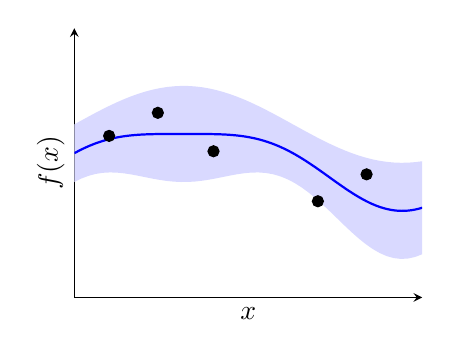
\begin{tikzpicture}
                \begin{axis}[
                    xlabel={$x$}, ylabel={$f(x)$},
                    ticks=none, axis lines=left,
                    ymin=-3, ymax=4, xmin=0, xmax=5,
                    height=5cm, width=6cm
                ]
                    \addplot[name path=A, draw=none, domain=0:5, samples=50] {sin(deg(x)) + 1.5};
                    \addplot[name path=B, draw=none, domain=0:5, samples=50] {sin(deg(x)) - 0.5 + 0.5*cos(deg(x)*2)};
                    \addplot[fill=blue!15, draw=none, forget plot] fill between[of=A and B];
                    \addplot[blue, thick, domain=0:5, samples=100] {sin(deg(x)) + 0.5 + 0.25*cos(deg(x)*2)};
                    \addplot[only marks, mark=*, mark size=2pt] coordinates {(0.5, 1.2) (1.2, 1.8) (2.0, 0.8) (3.5, -0.5) (4.2, 0.2)};
                \end{axis}
            \end{tikzpicture}
            }

            \vspace{0.3em}
            \scriptsize{
            Kernel:
            \[
            k(x, x') = \sigma_f^2 \exp\!\left(-\frac{\|x - x'\|^2}{2\ell^2}\right)
            \]
            Predictive mean \& variance:
            \begin{align*}
            \mu(x^*) &= k_*^\top (K + \sigma_n^2 I)^{-1} \mathbf{y} \\
            \sigma^2(x^*) &= k(x^*, x^*) - k_*^\top (K + \sigma_n^2 I)^{-1} k_*
            \end{align*}
            }
        \end{column}
        % --- Right Column: BAL ---
        \begin{column}{0.55\textwidth}
            \centering
            \textbf{2. Bayesian Active Learning (BAL)}

            \vspace{0.2em}
            \small{
            \[ \alpha(x) = \underbrace{\mu(x)}_{\text{Exploit}} + \kappa \cdot \underbrace{\sigma(x)}_{\text{Explore}} \]
            }

            \includegraphics[width=\linewidth, keepaspectratio]{bal.png}

            \vspace{0.5em}
            \footnotesize{\textit{We simulate points that maximize this score, reducing computational cost by orders of magnitude.}}
        \end{column}
    \end{columns}
\end{frame}
\begin{comment}
    
% Slide 1: Theory and Prediction Equations
\begin{frame}{Gaussian Process Regression: Theory}
  \begin{columns}
    % --- Left Column: Text and Math ---
    \begin{column}{0.58\textwidth}
      \footnotesize 
      \begin{itemize}
        \item \textbf{Definition:} A GP is a collection of random variables with a joint Gaussian distribution:
          \[
          f(\mathbf{x}) \sim \mathcal{GP}\big(m(\mathbf{x}),\, k(\mathbf{x},\mathbf{x}')\big).
          \]
        \item \textbf{Regression:} Given $\mathcal{D} = \{(\mathbf{x}_i,y_i)\}_{i=1}^{n}$, the posterior for a new $\mathbf{x}_*$ is:
          \[
          f_* \mid \mathbf{x}_*, \mathcal{D} \sim \mathcal{N}(\mu_*, \sigma^2_*).
          \]
        \item \textbf{Predictive Equations:}
          \begin{align*}
            \mu_* &= \mathbf{k}_*^\top (\mathbf{K} + \sigma_n^2 \mathbf{I})^{-1}\mathbf{y}, \\
            \sigma^2_* &= k_{**} - \mathbf{k}_*^\top (\mathbf{K} + \sigma_n^2 \mathbf{I})^{-1}\mathbf{k}_*.
          \end{align*}
      \end{itemize}
    \end{column}

    % --- Right Column: The Graph ---
    \begin{column}{0.42\textwidth}
      \centering
      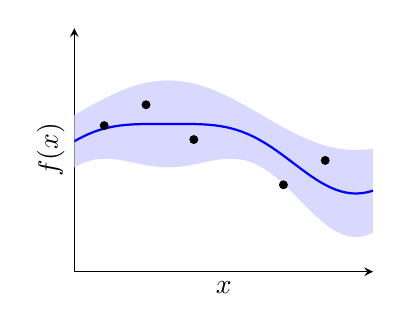
\begin{tikzpicture}[scale=0.7]
        \begin{axis}[
            xlabel={$x$},
            ylabel={$f(x)$},
            ticks=none,
            axis lines=left,
            ymin=-3, ymax=4,
            xmin=0, xmax=5,
            height=6cm, width=7cm,
            legend style={
              at={(0.5,-0.25)},
              anchor=north,
              font=\tiny,
              cells={align=left}
            },
            legend columns=3,
        ]
          % 1. UNCERTAINTY BAND (background)
          \addplot[name path=A, draw=none, domain=0:5, samples=50] {sin(deg(x)) + 1.5}; 
          \addplot[name path=B, draw=none, domain=0:5, samples=50] {sin(deg(x)) - 0.5 + 0.5*cos(deg(x)*2)};
          \addplot[fill=blue!15, draw=none, forget plot] fill between[of=A and B];

          % 2. MEAN LINE
          \addplot[blue, thick, domain=0:5, samples=100, forget plot]
            {sin(deg(x)) + 0.5 + 0.25*cos(deg(x)*2)};

          % 3. DATA POINTS
          \addplot[only marks, mark=*, mark size=2pt, color=black, forget plot] coordinates {
            (0.5, 1.2) (1.2, 1.8) (2.0, 0.8) (3.5, -0.5) (4.2, 0.2)
          };

    

        \end{axis}
      \end{tikzpicture}
    \end{column}
  \end{columns}
\end{frame}


%%%%%%%%%%%%%%%%%%%%%%%%%%%%%%%%%%%%%%%%

\begin{frame}
\frametitle{Bayesian Active Learning}

\begin{figure}[t!]
    \centering
    \includegraphics[width=0.8\textwidth]{bal.png}
    %\caption{Caption}
    \label{fig:my_label}
\end{figure}

\begin{scriptsize}
\begin{itemize}
    \item Training of standard GPs scales as $\mathcal{O}(N^3)$ with the number of observations $N$. \item Runtime consequently would increase drastically with increasing $N$.
    \item Bayesian active learning: ``add points where needed the most" (via a score function).
\end{itemize}

\begin{equation}
U(\tilde{x})=\sigma_m \tilde{\mu}(\tilde{x}) + \frac{\sigma_v}{2} \log \left(\tilde{\sigma}(\tilde{x}) \right)
 \label{eqn:Bayes_score}
\end{equation}
%
$\sigma_m>0$, $\sigma_v>0$, and where $\tilde{\mu}$ and $\tilde{\sigma}$ are the predictive mean and variance of a GP, trained at input locations ${\bf{X}}=\{x_1,...,x_n \}$, 
and evaluated at $\tilde{x}$, respectively. $\rightarrow $Fit a GP over the Welfare function (as a function of its parameters).

\end{scriptsize}
\end{frame}
\end{comment}


\begin{comment}
    
%%%%%%%%%%%%%%%%%%%%%%%%%%%%%%%%%%%%%%%%%%%%%%%%%%%%%
\begin{frame}{Bayesian Active Learning with Gaussian Processes}
%%%%%%%%%%%%%%%%%%%%%%%%%%%%%%%%%%%%%%%%%%%%%%%%%%%%%
\textcolor{blue}{\bf{$\rightarrow$ Uniform sampling in a high-dimensional space to populate the training set might be inefficient}}.
\vspace{0.4}

\begin{itemize}
    \item \textbf{Goal}: Given a fixed computational budget, efficiently approximate functions using GPs by \textcolor{blue}{actively selecting data points that improve the model’s accuracy}.
    \vspace{0.4}
    \item \textbf{Core Idea}: Rather than uniformly sampling, \textcolor{blue}{BAL strategically adds observations in areas where they contribute most to the model's performance} (e.g.,~\cite{rennerscheidegger_2018}, and references therein).   
    \vspace{0.4}
    \item \textbf{Application}: Particularly useful in settings like value function iteration, where acquiring \textcolor{blue}{\bf{new data points is computationally costly}} (each training sample consists of solving a constrained optimization problem). 
\end{itemize}
\end{frame}

%%%%%%%%%%%%%%%%%%%%%%%%%%%%%%%%%%%%%%%%%%%%%%%%%%%%%
\begin{frame}{How Bayesian Active Learning Works}
%%%%%%%%%%%%%%%%%%%%%%%%%%%%%%%%%%%%%%%%%%%%%%%%%%%%%
\begin{enumerate}
    \item \textbf{Model Update}: Fit a GP to current data \( \mathcal{D} = \{\mathbf{X}, \mathbf{y}\} \) to obtain a posterior mean and uncertainty for each point.
    \item \textbf{Acquisition Function}: Evaluate candidate points by their expected contribution to the model, often using a score like:
    \[
        \alpha(\tilde{x}_j; \mathcal{D}) = \sigma_m \tilde{\mu}(\tilde{x}_j) + \frac{\sigma_v}{2} \log \left(\tilde{\sigma}(\tilde{x}_j)\right)
    \]
    \item \textbf{Data Selection}: Select the candidate with the highest score, add it to the dataset, and update the model.\footnote{For effective use of the acquisition function, one needs to **randomly sample a set of candidate points** (e.g., 100), rank them by their acquisition scores, and add the highest-ranked point(s) to the training set.}
\end{enumerate}
\end{frame}
\end{comment}

%%%%%%%%%%%%%%%%%%%%%%%%%%%%%%%%%%%%%%%%%%%%%%%%%%%%%


\begin{frame}{Constructing the Welfare Surrogate}

    \begin{columns}[t]
    
        % --- Column 1: The Setup (UPDATED) ---
        \begin{column}{0.32\textwidth}
            \begin{block}{1. The Mapping}
                \small
                We map policy rules directly to \textbf{Expected Welfare}:
                \[
                    \vartheta \longmapsto \mathbb{E}_0[\mathcal{W}(\vartheta)]
                \]
                \begin{itemize}
                    \item \textbf{Input ($\vartheta$):} Tax and transfer parameters.
                    \item \textbf{Target:} Monte Carlo mean of lifetime utilities.
                \end{itemize}
            \end{block}
        \end{column}

        % --- Column 2: Smart Sampling ---
        \begin{column}{0.32\textwidth}
            \begin{block}{2. Active Training}
                \small
                We populate the training set $\mathcal{D}$ efficiently:
                \vspace{0.5em}
                \begin{itemize}
                    \item \textbf{Initial Design:} 450 points sampled randomly (Latin Hypercube).
                    \item \textbf{Refinement:} 50 points added via \textcolor{blue}{Bayesian Active Learning (BAL)}.
                    \item \textbf{Total:} Only 500 simulations needed.
                \end{itemize}
            \end{block}
        \end{column}

        % --- Column 3: The Model ---
        \begin{column}{0.32\textwidth}
            \begin{block}{3. The Model}
                \small
                Fitting the Gaussian Process:
                \vspace{0.5em}
                \begin{itemize}
                    \item \textbf{Kernel:} Squared Exponential with Automatic Relevance Detection (ARD).
                    \item \textbf{Accuracy:} Leave-One-Out (LOO) error $\approx \mathbf{10^{-4}}$.
                    \item \textbf{Result:} A smooth, cheap-to-query surface.
                \end{itemize}
            \end{block}
        \end{column}

    \end{columns}

\end{frame}
%%%%%%%%%%%%%%%%%%%%%%%%%%%%%%%%%%%%%%%%%%%%%%%%%%%%%
\begin{comment}
    
\begin{frame}
\frametitle{Hyperparameters to fit the Gaussian Process}
\begin{table}[h]
    \centering
    \begin{tabular}{|l|l|}
    \hline
    \textbf{Hyperparameter} & \textbf{Value} \\
    \hline
    Optimizer (LR) & Adam (0.01) \\
    $N_{samples}$ & 500 (450 + 50 BAL) \\
    kernel & Square Exponential kernel with Automatic Relevance Detection  \\
    \hline
    \end{tabular}
    \caption{Hyperparameters to fit the Gaussian process.}
    \label{tab:gp_params}
\end{table}

\end{frame}
\end{comment}

%%%%%%%%%%%%%%%%%%%%%%%%%%%%%%%%%%%%%%%%%%%%%%%%%%%%%
\subsection[3. Finding the Optimal Tax]{3. Finding the Optimal Tax}

{\setbeamercolor{background canvas}{bg=uzhgreylight}
\begin{frame}
\Huge \textcolor{uzhblue}{Finding the Optimal Tax}
%\begin{figure}
%    \centering
%    \includegraphics[width=0.5\textwidth]{IAM.png}
%    \caption{Caption}
%    \label{fig:enter-label}
%\end{figure}
\end{frame}}

\begin{frame}{Maximizing Welfare}
\begin{itemize}
    \item We now have a cheap-to-evaluate surrogate model to map \textcolor{blue}{tax functions onto welfare}. But we still need to find the optimal tax. 
    \vspace{0.5cm}
    \item We aim to \textcolor{blue}{find the $\argmax$ of our surrogate model}, which gives us the optimal tax function parameters: 
    \[
       \vartheta^* = \argmax_{\vartheta} \widehat{\mathrm{QoI}}(\vartheta)
    \]
    s.t. various constraints. 
    \vspace{0.5cm}     
    \item We use \textcolor{blue}{constrained optimization with linear constraints} for periods \{0,T\} that ensure that the parameters of the tax function stay within the feasible range during optimization.
    \end{itemize}
\end{frame}

%%%%%%%%%%%%%%%%%%%%%%%%%%%%%%%%%%%%%%%%%%%%%%%%%%%%%
\section [Results]{ Results}

{\setbeamercolor{background canvas}{bg=uzhgreylight}
\begin{frame}
\Huge \textcolor{uzhblue}{ Results}
%\begin{figure}
%    \centering
%    \includegraphics[width=0.5\textwidth]{IAM.png}
%    \caption{Caption}
%    \label{fig:enter-label}
%\end{figure}
\end{frame}}

%%%%%%%%%%%%%%%%%%%%%%%%%%%%%%%%%%%%%%%%%%%%%%%%%%%%%%%%
\begin{frame}[fragile]{Calibration}
\begin{table}[]
    \centering
    \begin{tabular}{ccc}
    \hline \hline
  \textbf{Symbol} & \textbf{Parameter} & \textbf{Value} \\
    \hline
    $\beta$  & Discount factor& 0.9 \\
    $\sigma$  & Relative risk aversion & 3 \\
    $\alpha$  & Capital share & 0.3 \\
    $\delta$  &Depreciation & 0.2 \\
    $\sigma_{ccr}$  & Climate sensitivity & 1.7 \\
    $\psi_1$  & parameter damage function & 13.16 \\
    $\theta_1$  & Intercept of control cost function & 0.7 \\
    $\theta_2$  & Exponent of control cost function & 2.6 \\
    $\kappa_{0}$  & Initial carbon intensity & 0.35032 \\
    $\rho_0$  & Initial AR(1) param for carbon intensity & 1.08 \\
    $\rho_{\infty}$  & Final AR(1) param for carbon intensity & 0.91 \\
    $\delta^{\rho}$  & AR(1) param depreciation for carbon intensity  & 0.04 \\
    $E_0$ & initial stock of carbon thGtC& 0.851 \\
    $L$ & Labor (to match initial emissions) & 600 \\
    \hline
\end{tabular}
    \caption{Parameterization of the OLG Model.}
    \label{tab:parameters}
\end{table}

\end{frame}
%%%%%%%%%%%%%%%%%%%%%%%%%%%%%%%%%%%%%%%%%%%%%%%%%%%%%%%%%%%%%%%%%%%%%
\begin{frame}{BAU Scenario versus RCP Scenarios}

    \centering
    % Image placed prominently at the top
    \includegraphics[width=0.9\textwidth, height=0.55\textheight, keepaspectratio]{BAU_SOLG.png}
    
    \vspace{1em}

    % Text split into columns to align with the "Left" and "Right" logic of the plots
    \begin{columns}[t]
    
        % Left Column: Emissions Description
        \begin{column}{0.48\textwidth}
            \footnotesize
            \textbf{Left: Global CO$_2$ Emissions}
            \begin{itemize}
                \item Comparison of our model's BAU against IPCC Representative Concentration Pathways (RCP).
                \item Our endogenous emissions path tracks closely with \textbf{RCP 4.5}.
                \item Base year (0) corresponds to 2017.
            \end{itemize}
        \end{column}

        % Right Column: Temperature Description
        \begin{column}{0.48\textwidth}
            \footnotesize
            \textbf{Right: Global Warming Projections}
            \begin{itemize}
                \item Projected mean warming reaches $\approx \mathbf{3^\circ C}$ over 150 years.
                \item Substantial uncertainty exists: range of \textbf{2.5°C to 3.6°C}.
                \item Highlights significant tail risk in the absence of policy.
            \end{itemize}
        \end{column}
        
    \end{columns}

\end{frame}

%%%%%%%%%%%%%%%%%%%%%%%%%%%%%%%%%%%%%%%%%%%%%
\begin{frame}{Three Policy Scenarios}
    \begin{itemize}
        \setlength\itemsep{1.2em}
        
        \item \textbf{Scenario 1: Unconstrained Welfare Maximization} \\
        \small{Linear tax on cumulative emissions + exogenous transfers.}
        \begin{equation*}
            \tau_t(E_t) = \vartheta_0 + \vartheta_E \cdot E_t
        \end{equation*}
        
        \item \textbf{Scenario 2: Pareto-Improving Policy} \\
        \small{Linear tax on cumulative emissions + \textbf{optimal} transfers.}
        \begin{equation*}
             \tau_t(E_t) = \vartheta_0 + \vartheta_E \cdot E_t
        \end{equation*}
        
        \item \textbf{Scenario 3: Increasing Policy Complexity} \\
        \small{Linear tax on cumulative emissions, carbon intensity ($\kappa$), and tipping risk ($TP$) + optimal transfers.}
        \begin{equation*}
            \tau_t(\cdot) = \vartheta_0 + \vartheta_E E_t + \vartheta_\kappa \kappa_t + \vartheta_{TP} (1-\mathbb{D}_{TP})
        \end{equation*}
    \end{itemize}
\end{frame}
%%%%%%%%%%%%%%%%%%%%%%%%%%%%%%%%%%%%%%%%%%%%%

%%

\begin{frame}{Scenario 1: Unconstrained Welfare Maximization}

 The youngest generation receives the largest share of total tax revenue, and the share for each older generation decreases by 10\% relative to the next younger one. The shares are normalized to sum to one. Formally, our transfer scheme, $\mathbb{T}$, is defined as:
%
\begin{equation}
    \mathbb{T}_{t,j} = 0.9^{(j-1)} \cdot 0.1394 \cdot \tau_t e_t, \quad j \in \{2,...,12 \}.
\end{equation}
The resulting constrained optimization problem reads as:
%
\begin{equation}
\label{eq:optim_cum_emm_maxwelf}
\begin{aligned}
  \vartheta^{\ast}
  \;=\;
  & \arg\max_{\vartheta\in[a,b]}\,
  \widehat{\mathrm{QoI}}(\vartheta) \\
& \quad \text{s.t.} \\
& 0 \leq \vartheta_0 + \vartheta_E  E_0 \leq \bar{\tau}, \\
& 0 \leq \vartheta_0 + \vartheta_E  E_{29} \leq \bar{\tau}.
\end{aligned}
\end{equation}
%
\end{frame}
%%%%%%%%%%%%%%%%%%%%%%%%%%%%%%%%%%%%%%%%%%%%%%
\begin{frame}{The Welfare Surrogate (Scenario 1)}

\begin{columns}[c]
    % Left Column: Image (given more space)
    \begin{column}{0.6\textwidth}
        \centering
        \includegraphics[width=\linewidth]{contour_welfare_E.pdf}
    \end{column}

    % Right Column: Minimal Text
    \begin{column}{0.4\textwidth}
        \small
      %  \textbf{Navigating the Policy Space:}
      %  \vspace{1em}
        \begin{itemize}
            \setlength\itemsep{1.5em}
            
            \item \textbf{The Surface:} A Gaussian Process approximation of the Social Welfare Function.
            
            \item \textbf{The Axes:} Tax Intercept ($\vartheta_0$) vs. Slope ($\vartheta_E$).
            
            \item \textbf{The Goal:} Find the "peak" (yellow zone) without running millions of simulations.
            
            \item \textbf{Precision:} Leave-One-Out error $\approx \mathbf{10^{-5}}$.
        \end{itemize}
    \end{column}
\end{columns}

\end{frame}


%%%%%%%%%%%%%%%%%%%%%%%%%%%%%%%%%%%%%%%%%%%%
\begin{frame}{Temperature (Scenario 1: Unconstrained)}

\begin{columns}[c]
    % Left Column: Image
    \begin{column}{0.55\textwidth}
        \centering
        \includegraphics[width=\linewidth]{Temp_case1.png}
    \end{column}

    % Right Column: The Explanation
    \begin{column}{0.45\textwidth}
        \small
        \textbf{Outcomes:}
        \begin{itemize}
            \setlength\itemsep{1em}
            
            \item \textbf{Aggressive Mitigation:} Stabilizes mean warming at \textbf{$\approx$2.7 °C}.
            
            \item \textbf{Tail-Risk Insurance:} The 99th percentile is capped at $\approx$3.1 °C.
            
            \item \textbf{The Mechanism:} Requires immediate, heavy taxation ($\approx$70\% average after 150 years).
            
            \item \textbf{The Cost:} Imposes up to \textbf{–5\% welfare losses} on current older cohorts.
        \end{itemize}
    \end{column}
\end{columns}

\end{frame}
%%%%%%%%%%%%%%%%%%%%%%%%%%%%%%%%%%%%%%%%%%%%
\begin{frame}{Emissions (Welfare Maximizing)}

\begin{columns}[c]
    \begin{column}{0.6\textwidth}
        \centering
        \includegraphics[width=\linewidth]{lin_S_10trans_unif_emissions.pdf}
    \end{column}

    \begin{column}{0.4\textwidth}
        \small
       % \textbf{The Physical Requirement:}
        \begin{itemize}
            \setlength\itemsep{1.2em}
            
            \item \textbf{Immediate Shock:} Emissions drop $\approx \mathbf{25\%}$ below BAU within the first 50 years.
            
            \item \textbf{Eliminating the Extremes:} The policy successfully truncates the high-emission tail (the red shaded area).
            
            \item \textbf{Convergence:} Post-2100, the gap narrows as exogenous carbon intensity declines naturally.
        \end{itemize}
    \end{column}
\end{columns}
\end{frame}
%%%%%%%%%%%%%%%%%%%%%%%%%%%%%%%%%%%%%%%%%%%%%%

\begin{frame}{Optimal Welfare Distribution}

\begin{columns}[c]
    \begin{column}{0.6\textwidth}
        \centering
        \includegraphics[width=\linewidth]{lin_S_10trans_unif_welfares.pdf}
    \end{column}

    \begin{column}{0.4\textwidth}
        \small
        \textbf{The Price:}
        \begin{itemize}
            \setlength\itemsep{1em}
            
            \item \textbf{Aggregate Welfare Gain:} The total pie grows by \textbf{1.6\%} (consumption equivalent).
            
            \item \textbf{Future Gain:} Generations born after 2100 enjoy gains of $\approx \mathbf{4.8\%}$.
            
            \item \textbf{Current Pain:} \textcolor{red}{This comes at a steep cost.} Transition generations suffer losses up to \textbf{5\%}.
            
            \item \textbf{Conclusion:} Without transfers, this optimal policy is politically dead on arrival.
        \end{itemize}
    \end{column}
\end{columns}
\end{frame}

%%%%%%%%%%%%%%%%%%%%%%%%%%%%%%%%%%%%%%%%%%%
\begin{frame}{The Challenge}
    \begin{itemize}
        \item The welfare-maximizing tax (simple example) reduces warming to $2.7^\circ$C.
        \item \textbf{But:} It imposes welfare losses of up to \textbf{5\%} on current older generations.
        \item \textbf{Result:} The policy is economically efficient but politically infeasible.
        \item \textbf{Goal:} Can we design a tax \textit{and} transfer scheme where $\tilde{U}_t \ge U_t$ for all $t$?
    \end{itemize}
\end{frame}
%%%%%%%%%%%%%%%%%%%%%%%%%%%%%%%%%%%%%%%%%%%

\begin{frame}{Scenario 2: Pareto-Improving Policy}
For 40 values of $t$:
\begin{equation}
    \mu_{*,t}(\vartheta) \;=\; \widehat{\mathrm{QoI}}_t(\vartheta)
  \;=\;
  \mathbb{E}\!\bigl[\tilde{U}_t(\vartheta)\bigr] \quad \forall \; t \in \{-10,...,29\}
\end{equation}

Solve:
\begin{equation}
\label{eq:opt_pareto_y2}
\begin{aligned}
  &\vartheta^{\ast}
  \;=\;
  \arg\max_{\vartheta\in[a,b]}
  \sum_{t=-10}^{29}\gamma_t\, \widehat{\mathrm{QoI}}_t(\vartheta)
  \;=\;
  \arg\max_{\vartheta\in[a,b]} 
  \sum_{t=-10}^{29}\gamma_t\,\mathbb{E}_0\!\bigl[\tilde{U}_t(\vartheta)\bigr] \\
& \quad \text{s.t.} \\ 
& \mathbb{E}_0\!\bigl[\tilde{U}_t(\vartheta)\bigr]
  \;\ge\;
  \mathbb{E}_0\!\bigl[U_t\bigr]
  \;\;\forall\,t, \\
& 0 \leq \vartheta_0 + \vartheta_E  E_0 \leq \Bar{\tau}, \\
& 0 \leq \vartheta_0 + \vartheta_E  E_{29} \leq \Bar{\tau},  \\
& \sum_{i=1}^{12} \vartheta_i = 1,
\end{aligned}
\end{equation}
\end{frame}

%%%%%%%%%%%%%%%%%%%%%%%%%%%%%%%%%%%%%%%%%%%%%
\begin{frame}{Optimal Parameters and Transfers}
We find optimal tax parameters: $\vartheta_0 = -0.186$ and $\vartheta_E = 0.225$.\newline

The optimal transfer shares allocate resources to specific cohorts to satisfy the Pareto constraints:

\begin{table}[htbp]
\begin{small}
        \centering
    \begin{tabular}{|c|c|c|c|c|c|c|c|c|c|c|c|c|}
        \hline
        \textbf{t1} & \textbf{t2} & \textbf{t3} & \textbf{t4} & \textbf{t5} & \textbf{t6} & \textbf{t7} & \textbf{t8} & \textbf{t9} & \textbf{t10} & \textbf{t11} & \textbf{t12} \\
        \hline
        0.128 & 0.051 & 0.058 & 0.09 & 0.15 & 0.09 & 0.066 & 0.143 & 0.076 & 0.048 & 0.039 & 0.06 \\
        \hline
    \end{tabular}
    \caption{\textbf{Pareto optimal transfer scheme.} Optimal shares for each concurrent cohort $i$ under the linear cumulative emissions tax.}
    \label{tab:optimal_transfer_lin_S}
    \end{small}
\end{table}
\end{frame}

%%%%%%%%%%%%%%%%%%%%%%%%%%%%%%%%%%%%%%%%%%%%%%%
\begin{frame}{Optimal Welfare (Pareto Improving)}

\begin{columns}[c]
    % Left Column: Image
    \begin{column}{0.6\textwidth}
        \centering
        \includegraphics[width=\linewidth]{welfare_gains_lin_S_trans.pdf}
    \end{column}

    % Right Column: Text
    \begin{column}{0.4\textwidth}
        \small
        %\textbf{Achieving Political Feasibility:}
        \begin{itemize}
            \setlength\itemsep{1em}
            
            \item \textbf{The Pareto Constraint:} Transfers are explicitly optimized to keep initial generations (and those born in the next decade) at \textbf{BAU levels} (0\% loss).
            
            \item \textbf{Future Gains:} Welfare improves monotonically, reaching \textbf{$\approx$1.4\%} for distant generations.
            
            \item \textbf{The Cost of Consensus:} Compared to the unconstrained case (max 4.8\%), future gains are smaller, but \textbf{no generation loses}.
            
            \item \textbf{Aggregate:} Total welfare gain of \textbf{0.42\%}.
        \end{itemize}
    \end{column}
\end{columns}

\end{frame}
%%%%%%%%%%%%%%%%%%%%%%%%%%%%%%%%%%%%%%%%%%%%%%%
\begin{frame}{Temperature (Scenario 2: Pareto-Improving)}

\begin{columns}[c]
    % Left Column: Image
    \begin{column}{0.55\textwidth}
        \centering
        \includegraphics[width=\linewidth]{Temp_case2.png}
    \end{column}

    % Right Column: The Explanation
    \begin{column}{0.45\textwidth}
        \small
       % \textbf{Political Viability:}
        \begin{itemize}
            \setlength\itemsep{1em}
            
            \item \textbf{The Trade-off:} Mean warming settles just below \textbf{3 °C} (higher than Scenario 1).
            
            \item \textbf{Crucial Insurance:} The 99th percentile \textbf{never exceeds 3.5 °C}.
            
            \item \textbf{Tail Truncation:} The policy deliberately eliminates the catastrophic tail ($>$3.6 °C under BAU).
            
            \item \textbf{The Win:} Achieved with optimal transfers $\to$ \textbf{no generation loses}.
        \end{itemize}
    \end{column}
\end{columns}

\end{frame}
%%%%%%%%%%%%%%%%%%%%%%%%%%%%%%%%%%%%%%%%%%%%%

\begin{frame}{Emissions: Mitigating Risk}
\begin{columns}
    \begin{column}{0.6\textwidth}
        \begin{figure}[th!]
            \centering
            \includegraphics[width=\linewidth]{lin_S_trans_emissions_dist.pdf}
        \end{figure}
    \end{column}
    \begin{column}{0.4\textwidth}
        \footnotesize
       % \textbf{Mechanism of Action:}
        \begin{itemize}
             \setlength\itemsep{1em} 
            \item \textbf{Modest Average Reduction:} The mean emissions path is not drastically lower than BAU (required to preserve current consumption).
            
            \item \textbf{Tail Truncation:} The policy's primary physical impact is eliminating the high-emissions upside.
            
            \item \textbf{Result:} The $99^{th}$ percentile of emissions drops below $40~GtCO_2$ by 2070 (20 years earlier than BAU).
            
            \item \textcolor{uzhblue}{\textbf{Conclusion:} The Pareto-optimal policy functions primarily as disaster insurance rather than aggressive mitigation.}
        \end{itemize}
    \end{column}
\end{columns}
\end{frame}
%%%%%%%%%%%%%%%%%%%%%%%%%%%%%%%%%%%%%%%%%%
\begin{frame}{Scenario 3: Increasing Policy Complexity}
    \textbf{Question:} Can we improve welfare by targeting specific climate drivers?
    \vspace{0.5em}
    
    We expand the tax rule to include \textbf{Carbon Intensity} ($\kappa_t$) and \textbf{Tipping Risk} ($TP_t$):
    
    \begin{equation}
        \label{eq:tax_fun_lin_S_kappa_tipping}
        \tau_t = \vartheta_0 + \vartheta_E \frac{E_t}{E_0} + \underbrace{\vartheta_\kappa \frac{\kappa_t}{\kappa_0}}_{\text{Intensity}} + \underbrace{\vartheta_{TP} (1 - \mathbb{D}_{TP})}_{\text{Tipping Risk}}
    \end{equation}
    
    \begin{itemize}
        \item $\mathbb{D}_{TP} \in [0,1]$: Normalized distance to the tipping threshold.
        \item \textbf{Dimensionality:} This adds new pseudo-states, increasing the parameter space to $d_\vartheta = 16$ (4 tax parameters + 12 transfer shares).
        \item We use the same ML-based optimization to find the constrained Pareto-optimal policy.
    \end{itemize}
\end{frame}
%%%%%%%%%%%%%%%%%%%%%%%%%%%%%%%%%%%%%%%%%%%%%%%%
\begin{frame}{Results: Diminishing Returns to Complexity}
    We find the optimal parameters:
    \[
        \{\vartheta_0, \vartheta_E, \vartheta_\kappa, \vartheta_{TP} \} = \{-0.237,\;  0.203, \;  0.037, \;  0.012 \}
    \]
    
    \textbf{Key Finding:} Complexity adds very little welfare value.
    
    \begin{table}[h]
        \centering
        \begin{tabular}{lcc}
            \toprule
            \textbf{Policy Specification} & \textbf{Instruments} & \textbf{Welfare Gain*} \\
            \midrule
            Linear in Cumulative Emissions ($E_t$) & 2 & \textbf{0.42\%} \\
            Linear in $E_t, \kappa_t, TP_t$ & 4 & \textbf{0.45\%} \\
            \bottomrule
        \end{tabular}
        \caption{\footnotesize Aggregate welfare gains in consumption-equivalent terms.}
    \end{table}
    
    \begin{alertblock}{Conclusion:}
        A simple, well-designed tax on cumulative emissions captures \textbf{93\%} of the potential welfare gains. Adding complex state-dependencies provides only marginal benefits.
    \end{alertblock}
\end{frame}
%%%%%%%%%%%%%%%%%%%%%%%%%%%%%%%%%%%%%%%%%%%%%%%%%%%%%
\begin{frame}{The Cost of Political Feasibility}
    Comparing the physical outcomes of the two approaches reveals a crucial trade-off: \newline
    
    % Added [t] here to align columns at the top
    \begin{columns}[t] 
    
        \begin{column}{0.5\textwidth}
            \textbf{1. Welfare Maximizing} \\ (Unconstrained)
            \begin{itemize}
                \item \textcolor{blue}{Aggressive early mitigation.}
                \item Warming stabilizes at $\mathbf{\approx 2.7^\circ C}$.
                \item \textcolor{red}{Current generations lose (up to 5\%).}
            \end{itemize}
        \end{column}
        
        \begin{column}{0.5\textwidth}
            \textbf{2. Pareto Improving} \\ (Constrained)
            \begin{itemize}
                \item \textcolor{blue}{Slower initial mitigation path.}
                \item Warming stabilizes at $\mathbf{\approx 3.0^\circ C}$.
                \item \textcolor{green}{No generation loses.}
                \item \textbf{\textcolor{uzhorange}{Crucial: Truncates worst-case damages (insurance).}}
            \end{itemize}
        \end{column}
    \end{columns}
    
    \vspace{1em}

    \begin{alertblock}{Trade-off \& Insurance}
        Ensuring political support requires delaying some mitigation, leading to higher \textit{average} temperatures ($\approx +0.3^\circ C$). However, it successfully \textbf{eliminates extreme damage scenarios} ($>15\%$ of GDP), effectively insuring future generations against climate disasters.
    \end{alertblock}
\end{frame}

%%%%%%%%%%%%%%%%%%%%%%%%%%%%%%%%%%%%%%%%%%%%%%%%%%%%%
\section[Conclusion \& Next Steps]{Conclusion \& Next Steps}

%%%%%%%%%%%%%%%%%%%%%%%%%%%%%%%%%%%%%%%%%%%%%%%%%%%%%

%%%%%%%%%%%%%%%%%%%%%%%%%%%%%%%%%%%%%%%%%%%%%%%%%%%%%
\begin{comment}
    
\begin{frame}{Next Steps}
\begin{itemize}
    \item Analyze richer, non-linear tax functions, solve for the optimal tax, and construct the Pareto frontier. % without functional assumptions.
        \vspace{0.5cm}
        \item Optimal transfers in ``quadratic'' tax model (parametrized).
                \vspace{0.5cm}
        \item Based on high-dimensional model representation~\citep{eftekhari_2022}, determine dominant terms that are driving results.
%    \item Solve for the Pareto frontier, i.e. ``all" welfare weights $\rightarrow$ Build a second surrogate.
\end{itemize}
\end{frame}
\end{comment}
%%%%%%%%%%%%%%%%%%%%%%%%%%%%%%%%%%%%%%%%%%%%%%%%
\begin{frame}{Conclusion}
    \begin{columns}
        \begin{column}{0.6\textwidth} % Slightly wider for text to prevent wrapping
            \scriptsize
            \begin{itemize}
                \setlength{\itemsep}{1.5em} % Increased spacing between items

                \item \textbf{Methodological Contribution:} \\
                A scalable 3-step ML framework (\textcolor{blue}{DEQN + GP + Optimization}) to solve previously intractable, high-dimensional OLG-IAMs.

                \item \textbf{Core Policy Result:} \\
                Simple linear tax + Optimal transfers $\rightarrow$ \textbf{Pareto Improvement}. \\
                Yields \textbf{0.42\%} aggregate welfare gain.

                \item \textbf{Insight on Complexity:} \\
                Adding intensity \& tipping targets yields only marginal gains (to \textbf{0.45\%}). \textbf{Simple, implementable rules capture the vast majority of benefits.}

                \item \textbf{Broader Implications:} \\
                Provides a generic blueprint for optimal fiscal and climate policy design in complex heterogeneous-agent environments.
            \end{itemize}
        \end{column}

        \begin{column}{0.4\textwidth}
            \centering
            \includegraphics[width=\linewidth]{summary_happy.png}
        \end{column}
    \end{columns}
\end{frame}

%%%%%%%%%%%%%%%%%%%%%%%%%%%%%%%%%%%%%%%%%%%%%%%%%%%%%

{\setbeamercolor{background canvas}{bg=uzhgreylight}
\begin{frame}
\Huge \textcolor{uzhorange}{Questions?}
\end{frame}}


\appendix

%{\setbeamercolor{background canvas}{bg=uzhgreylight}
%\begin{frame}
%\Huge \textcolor{uzhorange}{Appendix}
%\end{frame}}
% \begin{frame}{Labor endowment}
%     \begin{figure}
%         \centering
%         \includegraphics[width=0.5\linewidth]{labendow.png}
%         \caption{labor endowment profile}
%         \label{fig:enter-label}
%     \end{figure}
% \end{frame}


\appendix

\begin{comment}
    
\begin{frame}[fragile]{Appendix: Linear Tax in Time: Details}
\begin{itemize}
  

    \item The pseudostates ranges are: 
        \vspace{0.5cm}
    \begin{itemize}
        \item $\theta_1 \in [0,0.55]$, then bounds are given by $\{0, p_0\}$ (time is 0, i.e., second term plays no role anyways).
            \vspace{0.5cm}
        \item $\theta_2 \in [-0.019,0.0105]$, start from the linear equation $\theta_1 + \theta_2 \cdot t = \tau_t$. Due to decreasing mitigation costs over time, $\Bar{\tau}_t$ decreases over time. To get the upper bound set $\theta_1 = 0$, then $\Bar{\theta_2} = \Bar{\tau}_{29}/29$. And vice versa for the lower bound set $\theta_1 = 0.55$, then $\underline{\theta_2} = (\underline{\tau_{29}} - \theta_1)/ 29$, with $\underline{\tau_{29}} = 0$. 
            
    \end{itemize}
\end{itemize}

\end{frame}
\end{comment}

%%%%%%%%%%%%%%%%%%%%%%%%%%%%%%%%%%%%%%%%%%%%%%%%%%%%%

\begin{frame}[fragile]{Appendix: Sampling Domain}
\begin{table}[ht!]
\centering
\begin{tabular}{lllll}
\toprule
Model & Planner Target & Parameter & $\underline{\vartheta_i}$ & $\bar{\vartheta_i}$ \\
\midrule
Linear in E & Max. Welfare & $\vartheta_0$     & -2.0   & 2.0   \\
            & Max. Welfare & $\vartheta_E$     & -2.0   & 2.0  \\
           & Max. Welfare & $\tau$         & 0.0  & 1.5  \\
            \midrule
%linear in E  & pareto      & $\theta_1$     & -0.5 & 0.1 \\
%            & pareto      & $\theta_2$     & -0.1 & 0.5 \\
%            & pareto & $\tau$     & 0.0  & 0.8 \\
%\midrule
Linear in E + Transfers & Pareto & $\vartheta_0$ & -0.5 & 0.1 \\
                        & Pareto & $\vartheta_E$ & 0.0    & 0.5 \\
                        & Pareto & $\tau$         & 0.0  & 0.8  \\
\midrule
Full linear + Transfers & Pareto & $\vartheta_0$     & -1.0   & 0.5 \\
                        & Pareto & $\vartheta_E$     & -0.5 & 1.0   \\
                        & Pareto & $\vartheta_\kappa$ & -0.6 & 0.6 \\
                        & Pareto & $\vartheta_{TP}$   & -1.0   & 1.0   \\
                        & Pareto & $\tau$         & 0.0  & 0.8  \\
\bottomrule
\end{tabular}
\caption{Parameter bounds across models and objectives. }
\label{tab:param_bounds_main}
\end{table}

\end{frame}
%%%%%%%%%%%%%%%%%%%%%%%%%%%%%%%%%%%%%%%%%%%%%%%%%%%%%

% \begin{frame}[fragile]{Appendix: Linear Tax in 4 states: Details}
% \begin{itemize}
%     \item The pseudostates ranges are: $\theta_1 \in [-2.0,2.0], \theta_2 \in [-1.0,1.5], \theta_3 \in [-2.0,2.0], \theta_4 \in [-3.0,3.0]$.
       
%     \item The bounds for the tax are $\tau_t \in [0,2]$.
%     \item We take the values from the BAU case to find an upper bound for $E_t$ and then put a set of linear restrictions for the parameters. The parameters jointly satisfy:
%     $$0 \leq \theta_1 + \theta_2  E_0  + \theta_3  \kappa_0 + \theta_4  \frac{1}{TP_0} \leq \Bar{\tau} $$
%     $$0 \leq \theta_1 + \theta_2  E_T  + \theta_3  \kappa_T + \theta_4  \frac{1}{TP_T} \leq \Bar{\tau} $$
%     with $\{E_0,E_T\} = \{0.851,1.9\}$, $\{\kappa_0,\kappa_T\} = \{0.35,0.05\}$ and $\{TP_0,TP_T\} = \{3.0,3.0\}$.
%     \item In case of Pareto improvement, we need additional restriction that each generation has higher welfare with the tax compared to BAU 
% \end{itemize}

% \end{frame}


% \begin{frame}{Appendix: Multitask GPs}
%   \hypertarget{appendixslide}{}
% \footnotesize
%   \begin{itemize}
%     \item Multitask Gaussian process (GP) regression based on \cite{bonilla2007multi}.
%     \item \textbf{Use Case:} Extension of single task GP that captures intertask correlation.
%     \item \textbf{Covariance Formulation:} The covariance between two data points (\(x, x'\)) and two tasks (\(i, j\)) is modeled as:
%   \end{itemize}
%   \[
%   k([x, i], [x', j]) = k_{\text{inputs}}(x, x') \times k_{\text{tasks}}(i, j)
%   \]
%   \begin{itemize}
%   \footnotesize
%     \item Where:
%       \begin{itemize}
%       \footnotesize
%         \item \( k_{\text{inputs}}(x, x') \) is a standard kernel function (e.g., Squared Exponential Kernel) operating on the input data.
%         \item \( k_{\text{tasks}}(i, j) \) represents the inter-task covariance.
%       \end{itemize}
%       \item Prediction equation of a new point $x_*$:
%         \[
%   \mu(\bm{x}_*) = (\bm{k}_l^f \otimes \bm{k}_{*}^{x})^T \bm{\Sigma}^{-1} \bm{y}, \quad \text{where } \quad \bm{\Sigma} = \bm{K}^f \otimes \bm{K}^x + \bm{D} \otimes \bm{I}
%   \]
%   \end{itemize}
%          \( \bm{k}_l^f \): \( l \)-th column of the task covariance matrix \( \bm{K}^f \).
         
%         \( \bm{k}_{*}^{x} \): Vector of input covariances between test point \( \bm{x}_* \) and training points.
        
%         \( \bm{K}^x \): Input covariance matrix between all training points.
        
%         \( \bm{D} \): \( M \times M \) diagonal matrix of task noise variances \( \sigma_l^2 \).
        
%          \( \bm{\Sigma} \): \( MN \times MN \) joint covariance matrix.
% \hyperlink{mainslide}{\beamerbutton{Back to Main Slide}}
% \end{frame}

%%%%%%%%%%%%%%%%%%%%%%%%%%%%%%%%%%%%%%%%%%%%%%%%%%%%%
\begin{frame}[allowframebreaks]{References}

  \bibliography{bib_econ}
  \bibliographystyle{apalike}
%\usepackage{natbib}
%\bibliographystyle{plainnat}  

\end{frame}

\end{document}